

\setcounter{section}{0}
%==========================================

%\section*{第一章:相对论重离子碰撞}


\chapter{绪论}
% To add a non numbered chapter
%\addcontentsline{toc}{第一章}{相对论重离子碰撞}
% To insert this section on the table of contents

\setcounter{section}{0}

\setcounter{figure}{0}
\setcounter{table}{0}
\setcounter{equation}{0}

% \bigskip
自人类诞生以来,人类就试图在用自己的方式理解这个世界。“我们的世界是由什么组成的?”是人类自古以来的一大疑惑。在古代,人们对这些问题有着很多朴素的回答,从古希腊的“土气火水”四元素说到中国古代的“金木水火土”五行说,古人用一种朴素的元素分类法将物质世界简单地分解成几种元素。随着科技的发展,人类对世界的认识也得到了进一步的加深。自16-17世纪开始的科学革命使得新的科学观替代了以前朴素的科学观。经典力学开始建立,人类开始真正的用科学的观念、方法和手段来研究我们所在的世界。到19世纪末20世纪初,经典物理学的框架已经基本完善,人们认为物理学的大厦已经落成,仅有两朵乌云笼罩在美丽而晴朗的天空中。然而正是这两朵乌云引发了一场物理学的革命。
随着爱因斯坦于1905年和1915年先后创立狭义相对论和广义相对论,经典物理学中的绝对时间和绝对空间的概念被打破。而光的波粒二象性的提出和量子力学的建立让人们开始对微观世界的运行方式有了新的认识。相对论和量子力学的建立标志着物理学从经典物理学时代走入了近代物理学时代,粒子物理也正是在这一时期成为了物理学研究的热门课题。

粒子物理是研究组成物质的基本粒子的一门学科,其研究的对象主要为物质的基本组成单元——各种基本粒子以及他们之间的相互作用。现如今,在粒子物理学界公认的最成功的描述电、弱、强相互作用的理论是标准模型(Standard Model, SM)。自上世纪七十年代理论成型以来,标准模型成功的经受住了许多实验的检验。2012年,随着LHC上的ATLAS和CMS合作组发现Higgs玻色子\cite{ATLAS:2012yve,CMS:2012qbp},标准模型的最后一块拼图被也已经被补全。标准模型的提出者Peter Higgs 和 Francois Englert也于2013年获得了诺贝尔奖。但标准模型绝不是一个“最终的”理论模型,仍有许多问题是标准模型没法解释的,例如暗物质、中微子质量、muon的反常磁矩等问题。这些问题就像是山那边的海一样吸引着人们去探索。或许在翻越一座座山峰之后,又一场颠覆我们现今认识的物理学革命在等着我们。

\section{标准模型}

正如上文提到的那样,标准模型是现在最为广泛接受的描述电、弱、强三种相互作用的理论。像门捷列夫的元素周期表一样,标准模型也成功的预言了许多粒子和现象,并且得到了实验的证实。标准模型中,基本粒子由轻子、夸克、规范矢量玻色子以及Higgs玻色子构成。如图 \ref{fig:ParticleTable} 所示
\begin{figure}[htb]
    \begin{center}
    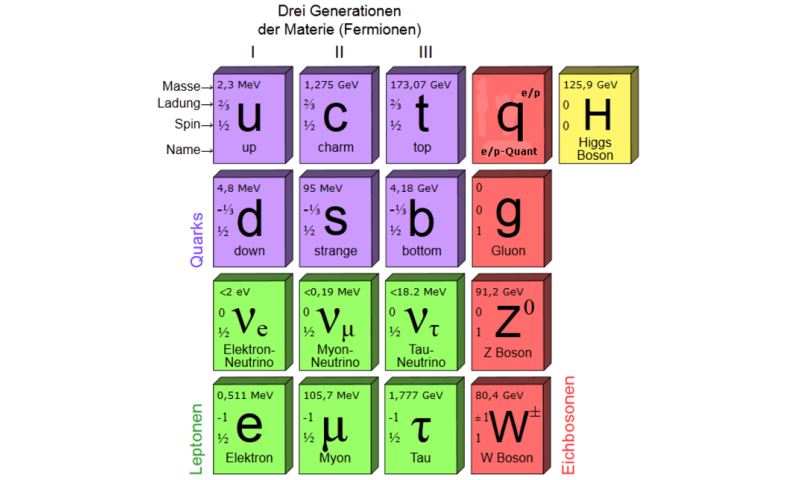
\includegraphics[width=\textwidth,clip]{figures/Chapter1/ParticleTable.png}
    \end{center}
    \caption[标准模型中的基本粒子]{标准模型中的基本粒子}
    \label{fig:ParticleTable}
\end{figure}
其中轻子和夸克为自旋为1/2的费米子,每一种轻子和夸克都有其对应的反粒子。轻子共分为三代(Generation),电子,muon,tau轻子和其对应的中微子分别组成不同的代。每一代轻子和其反粒子都带有被称为轻子数的量子数,轻子严格地遵守轻子数守恒定律。夸克和轻子之间存在着某种对称性,自然,夸克也存在和轻子类似的代的概念,被分为三代夸克,如图 \ref{fig:ParticleTable}所示。除了自旋为1/2的费米子以外,标准模型中还存在着四种规范矢量玻色子作为费米子之间的相互作用的传播子存在。其中光子,$W^{\pm}$以及 $Z^0$玻色子为自旋为1的粒子,而Higgs玻色子为目前唯一自旋为0的玻色子。他的引入源于解决弱相互作用的对称性破缺问题时引入的Higgs场,当粒子与Higgs场相互作用的时候其不再以光速进行传播并且获得质量。而那些不与Higgs场有相互作用的粒子,例如光子、胶子等则保持质量为零。

在量子力学建立之初,人们只是用它来处理粒子这种物质的存在,而对于物理学中另一个很重要的概念——场却没有进行量子化的处理,仍然是经典的,并没有将其和粒子放在同等地位。这就导致有一些问题仍然无法得到很好的解决,例如光电效应、原子发射和吸收光子以及粒子的产生和湮灭等问题。这就让人们开始考虑将量子化的概念从单粒子拓展到场的范围。人们开始尝试把克莱因-高登和狄拉克方程解释成为场方程,即将其中的波函数解释为经典场,从而开始了场的量子化过程。在历史上人们首先对电磁场进行了量子化。得到了处理电磁场相互作用的理论,被称为量子电动力学(Quantum Electrodynamics, QED)。电磁相互作用的传播子为光子。

之后在处理中子的$\beta$衰变的时候,费米意识到电磁相互作用不可能产生这个过程,应该是由于某种新的相互作用而引起了中子的$\beta$衰变过程。这种新的相互作用就是弱相互作用。弱相互作用的强度远弱与电磁相互作用,比电磁相互作用弱了大约$10^{11}$倍。其传播子为$W^{\pm}$以及 $Z^0$。

1937年,汤川秀树类比于描写电磁相互作用的QED理论,提出核力是通过中子和质子之间的一种具有质量的基本粒子来传递的。基于此,汤川预言有一种新的粒子存在,其质量应该介于电子和质子之间,汤川将这种新粒子称为介子(Meson)。后来,汤川预言的这种粒子于1947年被发现,被称为$\pi$介子。至此,粒子世界的主要角色似乎已经齐全了。但在同一年,随着奇异粒子的发现,这种“齐全”的错觉被无情的打破,人们意识到现有的理论不足以解释越来越多的被发现的新粒子。这样人们就有了一个很自然的疑问:这些粒子是否还有着自己的内部结构?

之后夸克模型便被提出用以解释强子的结构问题。1964年由默里·盖尔曼和乔治·茨威格分别独立提出了夸克模型。其认为强子由三种基本的构造单元组成,这三种不同的构造单元被称为具有三种不同味(Flavor)的夸克(Quark),分别是u(up),d(down)和s(strange)夸克。夸克模型很好的解释了强子的生成和湮灭问题,但是在处理一些粒子的组分的时候遇到了困难。按照夸克模型,$\Omega^-$应该有三个s夸克组成且都处于轨道运动的基态,又因为$\Omega^-$的总自旋角动量为$\frac{3}{2}\hbar$,这就要求每一个s夸克的自旋都应该是$\frac{1}{2}\hbar$,明显的违背了泡利不相容原理。基于这个事实,人们开始猜测是否还有一种新的未知的量子数。1965年南部阳一郎研究了这个问题并提出夸克应该有一种新的量子数,他称之为色(Color),从此量子色动力学(Quantum Chremodynamics, QCD)走上了粒子物理学的舞台。


% \subsection{量子色动力学}
量子色动力学被用来描述强相互作用,其传播子为胶子(gluons)。拉式量(Lagrangian)可以表示为:
\begin{equation}
    \mathcal{L}_{QCD} = \bar{\phi}(i \gamma_{\mu} D^{\mu}-m)\phi-\frac{1}{2}G^{a}_{\mu\nu}G^{\mu\nu}_{a}
\end{equation}
其中
\begin{equation}
    G^{a}_{\mu\nu} = \delta_{\mu}A_{\nu}^{a}(x) - \delta_{\nu}A_{\mu}^{a}(x) + gf_{abc}A_{\mu}^{b}(x)A_{\nu}^{c}(x)
\end{equation}
$D^{\mu}$为夸克场与胶子场耦合的协变微分,形式为:
\begin{equation}
    D^{\mu} = \delta_{\mu} - ig\frac{\lambda_{a}}{2}A_{\mu}^{a}(x)
\end{equation}
其中g为QCD耦合常数,$f_{abc}$为$SU(3)_{color}$结构常数,$\phi$为夸克场(对夸克味求和),$\gamma_{\mu}$为狄拉克矩阵,$\lambda_{a}$为盖尔曼矩阵,$G^{a}_{\mu\nu}$为规范不变的场强张量,$A_{\mu}^{a}$为胶子场。量子色动力学有着一些独特的特性,将会在下文中进行介绍。

在自然界中,我们并不能观测到单个存在的夸克,我们只能观测到由多个夸克组成的色中性的强子态(准确的说是色单态)。这意味着夸克和胶子之间的相互作用在距离变远的时候会增长的极快,从而使单个的夸克或者胶子难以存在。在量子色动力学中,势能可以描述为
\begin{equation}
    V_s = -\frac{4}{3}\frac{\alpha_{s}}{r} + kr
    \label{eq:QCDpotential}
\end{equation}
其中$\alpha_{s}$为强相互作用的耦合常数。

第一项在距离较短的时候占主导作用,类似于QED当中的库伦势。随着距离的增加,第二项开始占据主导作用,夸克和胶子之间的作用力成近似线性增加。在深度非弹散射(Deep Inelastic Scattering, DIS)实验中人们发现强子中的夸克和胶子表现出来准自由点状粒子的性质,而根据式\ref{eq:QCDpotential},当r趋近于零的时候$V_s$应该趋近于无穷,这就是知名的朗道极点问题。这个问题在量子色动力学中被由大卫·格罗斯、弗兰克·维尔切克和大卫·波利策提出的渐进自由理论解决。

重整化后的强相互作用力有效耦合常数可以写作:
\begin{equation}
    \alpha_{s}(|q^2|) \equiv \frac{g_s^2(|q^2|)}{4\pi} \approx \frac{12\pi}{\beta_0 ln(|q^2|/\Lambda_{QCD}^2)}
\end{equation}
其中 $\beta_0 = (11n_c-2n_f)$为一个由夸克的颜色数目 $n_c$ 和 夸克的味道数目$n_f$给出来的常数。因为$\beta_0 > 0$,所以$\alpha_{s}$随着$|q^2|$的增加而减小,这显示出来了渐进自由的特性。在实验上可以在不同的能量尺度($Q^2$)的情况下测量强相互作用的耦合常数,其行为和预测的相同,实验上的测量结果如图 \ref{fig:Alpha_S} 所示
\begin{figure}[htb]
    \begin{center}
    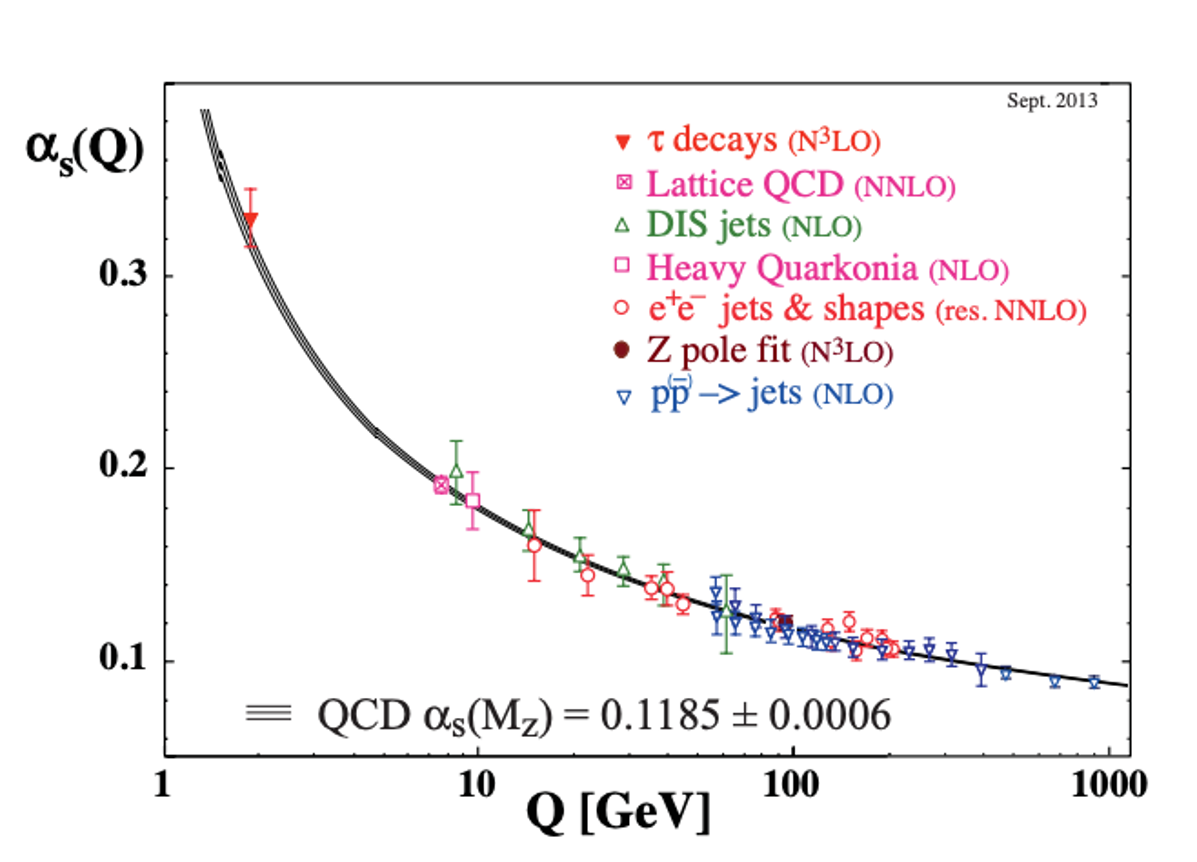
\includegraphics[width=0.7\textwidth,clip]{figures/Chapter1/Alpha_s.png}
    \end{center}
    \caption[$\alpha_s$随能量尺度$Q^2$变化的关系]{$\alpha_s$随能量尺度$Q^2$变化的关系,2014 review of paritcles}
    \label{fig:Alpha_S}
\end{figure}

渐进自由带来了几个有趣的结果。首先在大$Q^2$区间,$\alpha_s \ll 1$。这使得微扰理论在此能量尺度下仍然可以起作用。但随着$Q^2$的减小,$\alpha_s \geq 1$,从而使得微扰量子色动力学不再适用。因此其他的理论被发展出来在此区间进行量子色动力学的计算。目前比较成功的非微扰量子色动力学的计算方式为格点量子色动力学(Lattice QCD)。
% \subsection{渐进自由}
在自然界中,我们并不能观测到单个存在的夸克,我们只能观测到由多个夸克组成的色中性的强子态(准确的说是色单态)。这意味着夸克和胶子之间的相互作用在距离变远的时候会增长的极快,从而使单个的夸克或者胶子难以存在。在量子色动力学中,势能可以描述为
\begin{equation}
    V_s = -\frac{4}{3}\frac{\alpha_{s}}{r} + kr
    \label{eq:QCDpotential}
\end{equation}
其中$\alpha_{s}$为强相互作用的耦合常数。第一项在距离较短的时候占主导作用,类似于QED当中的库伦势。随着距离的增加,第二项开始占据主导作用,夸克和胶子之间的作用力成近似线性增加。在深度非弹散射实验中人们发现强子中的夸克和胶子表现出来准自由点状粒子的性质,而根据式\ref{eq:QCDpotential},当r趋近于零的时候$V_s$应该趋近于无穷,这就是知名的朗道极点问题。这个问题在QCD中被由大卫•格罗斯,弗兰克•维尔切克和大卫•波利策提出的渐进自由理论解决。

重整化后的强相互作用力有效耦合常数可以写作:
\begin{equation}
    \alpha_{s}(|q^2|) \equiv \frac{g_s^2(|q^2|)}{4\pi} \approx \frac{12\pi}{\beta_0 ln(|q^2|/\Lambda_{QCD}^2)}
\end{equation}
其中 $\beta_0 = (11n_c-2n_f)$为一个由夸克的颜色数目 $n_c$ 和 夸克的味道数目$n_f$给出来的常数。因为$\beta_0 > 0$,所以随着$|q^2|$的增加而减小,这显示出来了渐进自由的特性。在实验上可以在不同的能量尺度($Q^2$)的情况下测量强相互作用的耦合常数,其行为和预测的相同,实验上的测量结果如图 \ref{fig:Alpha_S} 所示
\begin{figure}[htb]
    \begin{center}
    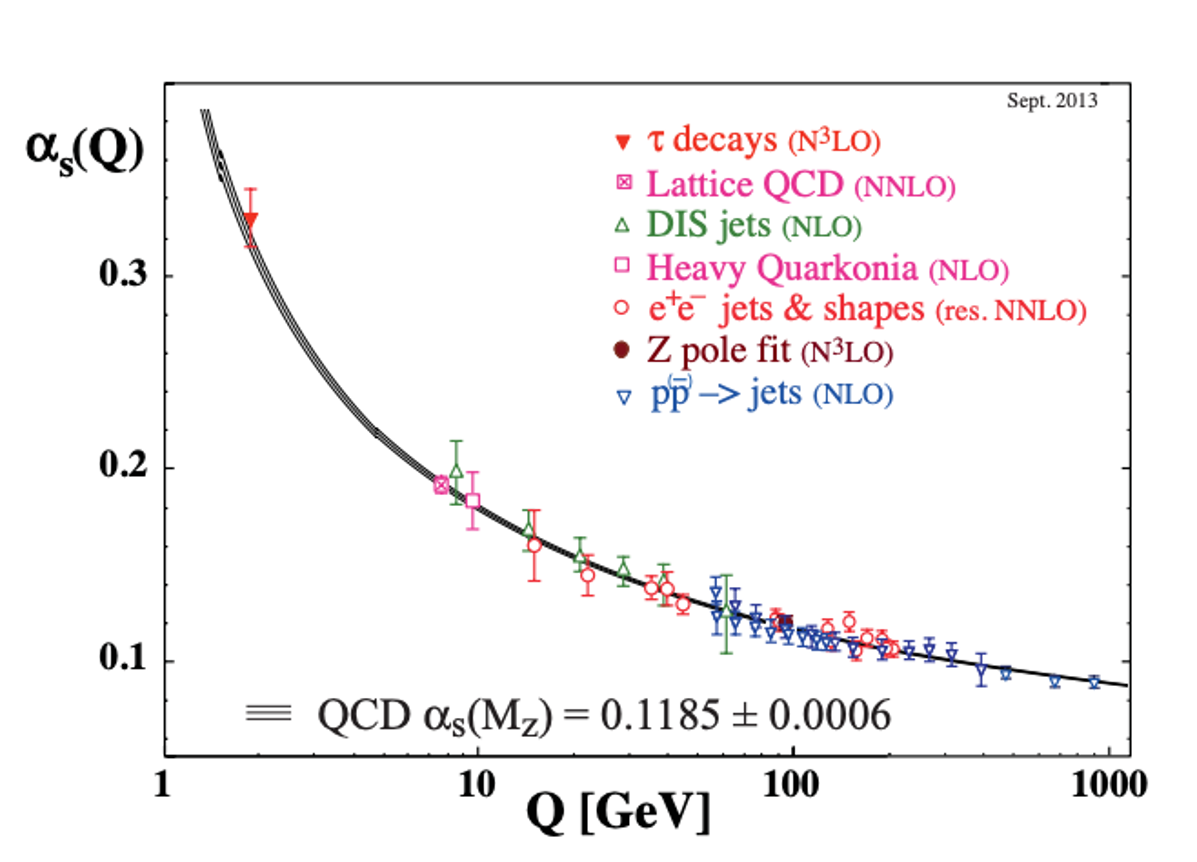
\includegraphics[width=\textwidth,clip]{figures/Chapter1/Alpha_s.png}
    \end{center}
    \caption[$\alpha_s$随能量尺度$Q^2$变化的关系]{$\alpha_s$随能量尺度$Q^2$变化的关系,2014 review of paritcles}
    \label{fig:Alpha_S}
\end{figure}

渐进自由带来了几个有趣的结果。首先在大$Q^2$区间,$\alpha_s \ll 1$。这使得微扰理论在此能量尺度下仍然可以起作用。但随着$Q^2$的减小,$\alpha_s \geq 1$从而使得微扰QCD不再适用。因此其他的理论被发展出来在此区间进行QCD的计算。目前比较成功的非微扰QCD的计算方式为格点QCD(Lattice QCD)。
\section{夸克胶子等离子体}
\label{夸克胶子等离子体}
因为量子色动力学渐进自由的性质,在极端高温下或者密度极高的情况下夸克和胶子可能解禁闭形成新的物质态。类似于等离子体中的电子和原子之间的束缚在高温或者高密的情况下被解除紧闭,电子可以在等离子体中自由移动从而带来很高的电导率一样。在这种新的物质态当中束缚夸克和胶子的强相互作用力被屏蔽,从而使得夸克从强子束缚态中解紧闭形成一种类似于等离子体的状态。这种新的物质的态被称作夸克胶子等离子体(Quark Gluon Plasma, QGP)。根据格点量子色动力学预言,在高温和(或)高密的情况下物质可能发生从强子气到夸克胶子等离子体的相变。和其他物质的相变类似,这种从强子气到夸克胶子等粒子体的相变也有属于自己的相图,如图 \ref{fig:PhaseDiagram} 所示

\begin{figure}[htb]
    \begin{center}
    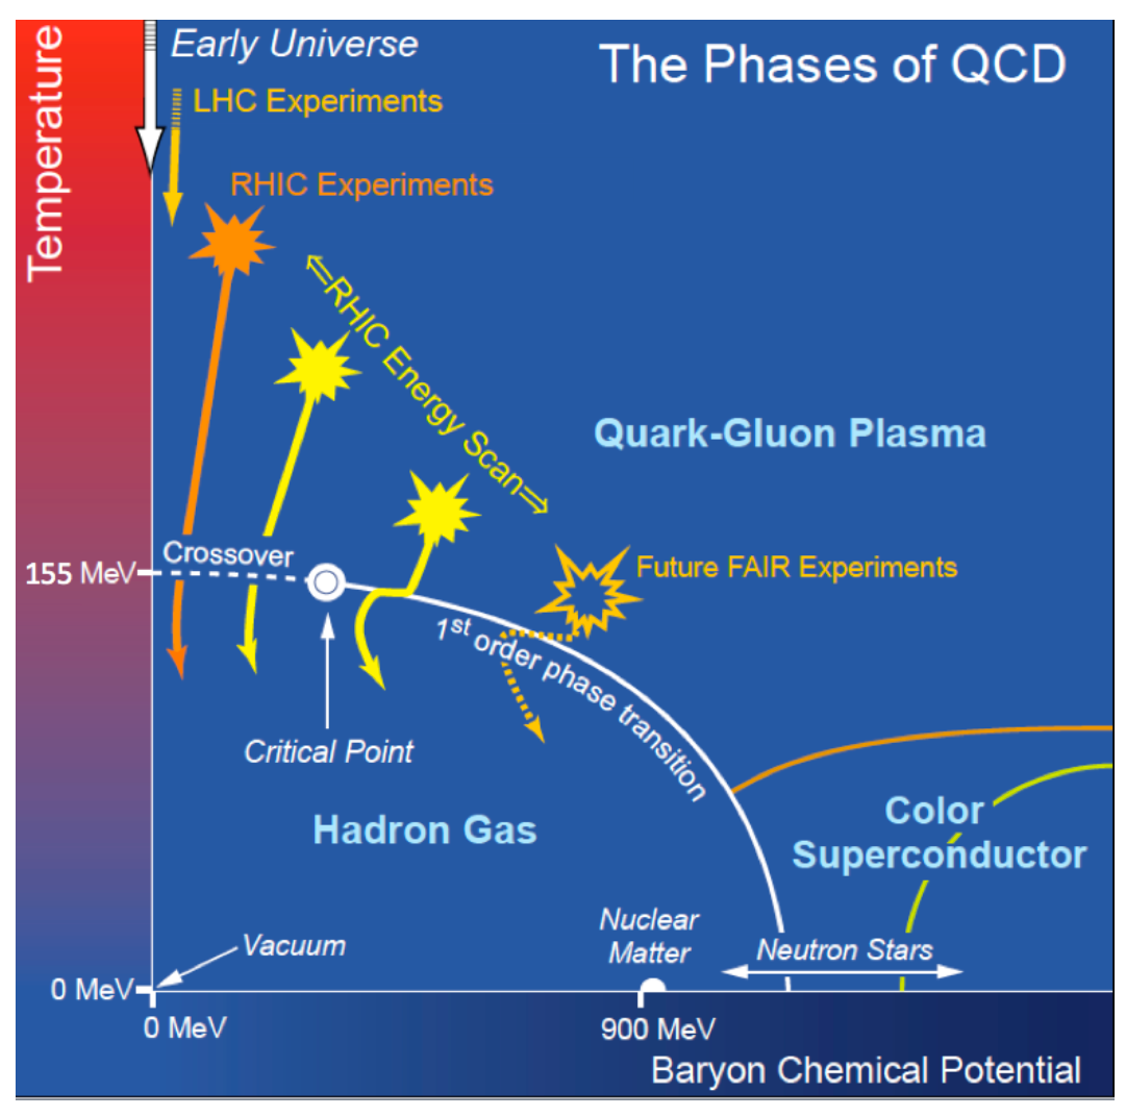
\includegraphics[width=0.7\textwidth,clip]{figures/Chapter1/PhaseDiagram.png}
    \end{center}
    \caption[QGP相图]{QGP相图}
    \label{fig:PhaseDiagram}
\end{figure}

量子色动力学相图给出来的是在温度T和重子化学势$\mu_b$平面上的热力学状态图,从图中可以看出,研究量子色动力学物质相变时,有两种常见的路线。一种是在保持低温的情况下增加夸克物质的密度,沿着这条路线最后达到的物质状态即为中子星内部的物质状态。另一条路线是加热核物质,也可以达到从强子气到夸克胶子等粒子体的相变,这种方式一般通过相对论重离子对撞来实现。
\section{手征对称性}

量子色动力学的拉氏量除了拥有$SU(3)_{color}$和$SU(3)_{flavor}$近似对称性以外还存在着另外一种对称性——手征对称性

当动量转移$Q \sim 1 {\rm~GeV/c}$的时候三种最轻的夸克,上、下和奇异夸克可以被近似地认为质量为零。在这种情况下拉氏量可以被写为:
\begin{equation}
    \label{QCDLagrangian}
    \mathcal{L} = i\bar{\phi}_f \gamma^{\mu} \delta_{\mu} \phi_{f}
\end{equation}

其中f表示夸克的味道。此拉氏量的一个重要的性质是在矢量和轴矢量变换下都有对称性:

\begin{equation}
    \label{Vector}
    \phi \rightarrow e^{i \alpha^{a}_{V}\frac{\lambda_a}{2}} \phi
\end{equation}
\begin{equation}
    \label{AxialVector}
    \phi \rightarrow e^{i \gamma_5 \alpha^{a}_{A}\frac{\lambda_a}{2}} \phi
\end{equation}

矢量和轴矢量的波函数可以用他们的左手或者右手手征分量来表示:

\begin{equation}
    \phi_{R,L} = \frac{1}{2}(1 \pm \gamma_5) \phi
\end{equation}

当我们考虑手征分量的时候变换\ref{Vector}和\ref{AxialVector}可以表示为:

\begin{equation}
    \phi_R \rightarrow e^{i \gamma_5 \alpha^{a}_{R}\frac{\lambda_a}{2}} \phi_R~,~\phi_L \rightarrow \phi_L
\end{equation}
\begin{equation}
    \phi_L \rightarrow e^{i \gamma_5 \alpha^{a}_{L}\frac{\lambda_a}{2}} \phi_L~,~\phi_R \rightarrow \phi_R
\end{equation}

在矢量和轴矢量的变化下我们可以看到一个由手征分量构成的对称性,这种在夸克质量为零的条件下的$SU(N_f)_{R} \times SU(N_f)_{L}$对称性被称作手征对称性。

当夸克质量不为零的时候其可以为视为量子色动力学拉氏量\ref{QCDLagrangian}当中的一个微扰项($\delta\mathcal{L} = -m\bar{\phi}\phi$)。这个微扰项带来了在轴矢量变换下的对称性破缺,因此也打破了手征对称性。对称性破缺可以表现为显式的对称性破缺或者是自发对称破缺。在显式对称性破缺中,对称性的破缺表现为拉氏量在运动方程中对称破缺。但在自发对称破缺中,运动方程依旧保持不变,系统的对称性破缺表现在系统的基态并不是稳定的。

“墨西哥”帽的势能形象地展示了这种自发对称性破缺的状态,如图\ref{fig:MexHat}所示。在这个状态下系统十分的不稳定,任何微小的扰动都可能打破这种平衡,在图中表现为一个很小的扰动就可以让小球从“帽尖”出滑落。这种不稳定性来源于对称性的自发破缺,例如手征对称性。当三种夸克被看作质量为零的时候,我们期待有8种简并的无质量的Goldstone玻色子,其量子数为$J^P = 0^-$。但在实际上是有8种介子拥有此量子数,分别为$\pi^{\pm},\pi^0,K^{\pm},K^0,\bar{K}^0$和$\eta$,手征对称性的自发破缺导致了他们的非零质量。例如这些介子里面最轻的介子$\pi^0$的质量为 $m_{\pi^0} \approx 135~{\rm MeV/c^2}$,但最轻的包含s夸克的介子$K^{\pm}$质量为$m_{K^{\pm}} \approx 494~MeV/c^2$

\begin{figure}[htb]
    \begin{center}
    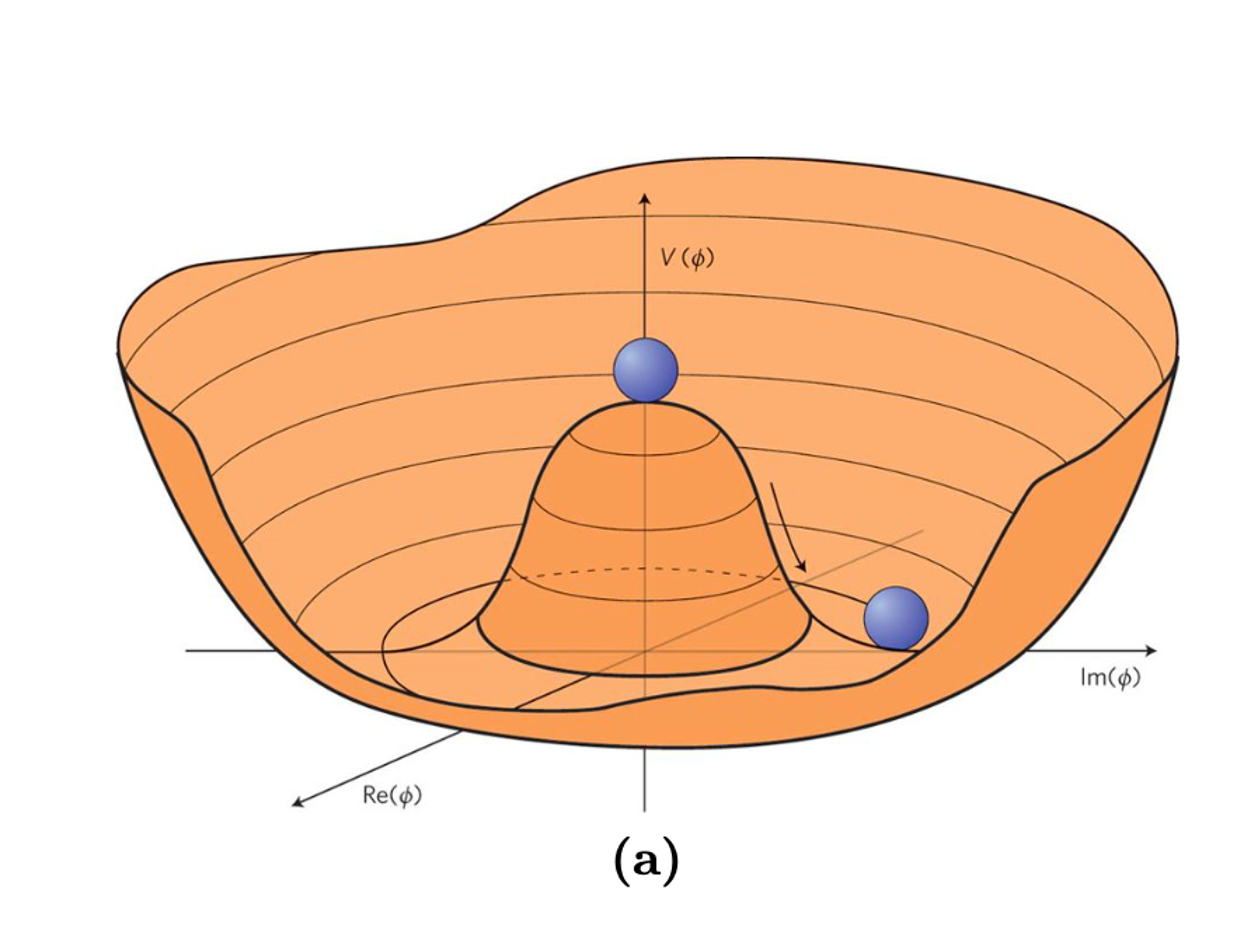
\includegraphics[width=0.7\textwidth,clip]{figures/Chapter1/MexHat.png}
    \end{center}
    \caption["墨西哥帽"势能示意图]{"墨西哥帽"势能示意图}
    \label{fig:MexHat}
\end{figure}

手征对称性的破缺也导致了真空中的夸克凝聚(quark condense)。可以从$\pi$介子的质量和夸克凝聚的关系(Gell-Mann-Oakes-Renner关系)中得到:

\begin{equation}
    m_{\pi}^2 f_{\pi}^2 = -2\bar{m}\langle 0|\bar{q}q|0 \rangle
\end{equation}
其中$\bar{m} \approx 6~ {\rm MeV/c^2} $是u和d夸克的平均质量。从这个关系式中我们可以看到真空中的夸克凝聚的值$\langle 0|\bar{q}q|0 \rangle \approx (-250 {\rm~MeV})^3$。这也是手征对称性破坏的标志之一。

在实验上对手征对称恢复的观测可以通过测量手征多重态的质量分布来做到,例如$\rho^0(770)$和$a_1(1260)$。如果没有手征对称性破缺这两个态将会是简并的,然而在实验的测量中却发现他们两个的质量差别很大:$m_{\rho^0} \approx 770 ~{\rm MeV/c^2}$, $m_{a_1} \approx 1260 ~{\rm MeV/c^2}$。这种质量的差别不能简单的被u夸克和d夸克的质量差别来描述,很可能由手征对称性的破缺带来。

人们预期这种夸克凝聚态会在高温($T > T_c^{chiral}$)、高密($n > n_c^{chiral}$)的条件下发生改变。因此人们期待在这种条件下可以看到从带有自发手征对称性破缺强子物质态到手征恢复的物质态的转变。但需要注意的是手征恢复的的相变条件和量子色动力学物质解禁闭的相变条件并不相同,人们预期手征对称恢复的相变温度要高于夸克胶子等离子体的相变温度,即在相同的重子势下,$T_c^{chiral} > T_c^{QGP}$。这就意味着夸克胶子等离子体可能在手征对称恢复没有达到的情况下存在,同时也意味着存在手征对称恢复的时候夸克和胶子一定是解禁闭的。在实验上手征对称恢复一个很重要的观测量便是$\rho^0$和$a_1$质量的简并,对他们质量谱的测量是我们直接对手征对称恢复进行观测的一个很重要的手段。

\section{相对论重离子对撞}

正如 \ref{夸克胶子等离子体} 一节中所提到的一样,在实验上产生夸克胶子等离子体的主要方式为相对论重离子对撞。通过控制相对论重离子对撞的离子类型和对撞中每核子对的能量($\sqrt{s_{NN}}$),可以在QCD的相图中得到不同的T-$\mu_b$曲线。从而成为探索QCD相图的有力的工具。以相对论重离子对撞机(Relativistic Heavy-Ion Collider, RHIC)为例。常用的对撞系统为金-金对撞,最高可以达到 \sNNerbai 的对撞能量,在这种情况下金离子可以被加速到大约99.99\%的光速。

在相对论情况下球状的原子核会收缩成扁平的盘状,当他们在束流管中交汇时就可能发生对撞。一个很重要的描述对撞对心程度的参数为碰撞参数b,其定义为两个核中心之间的距离,参见图 \ref{fig:ImpactParameter}。当$b \approx 0$时称为“中心(Central)”对撞,当$b \approx 2R$时称为“偏心(Peripheral)”对撞。但在实验上我们无法直接观测到一次对撞发生时的碰撞参数,所以我们用一个基于带电粒子多重数(在某区间内的带电粒子数,Reference Multiplicity,RefMult)的中心度(Centrality)定义来描述对撞的对心程度。Glauber模型被用来计算对撞发生后带电粒子多重数的分布,在Glauber模型中带电粒子多重数和中心度关系的示意图见图 \ref{fig:Centrality}。除了中心度,还有一些常用的量也被用来描述对撞的对心程度,例如参加对撞核子数($N_{part}$),二元碰撞数($N_{bin}$)以及核几何重叠函数(Geometrical nuclear overlap function, $T_{AA} = N_{coll}/\sigma_{NN}^{inel}$)等。

\begin{figure}[htb]
    \begin{center}
    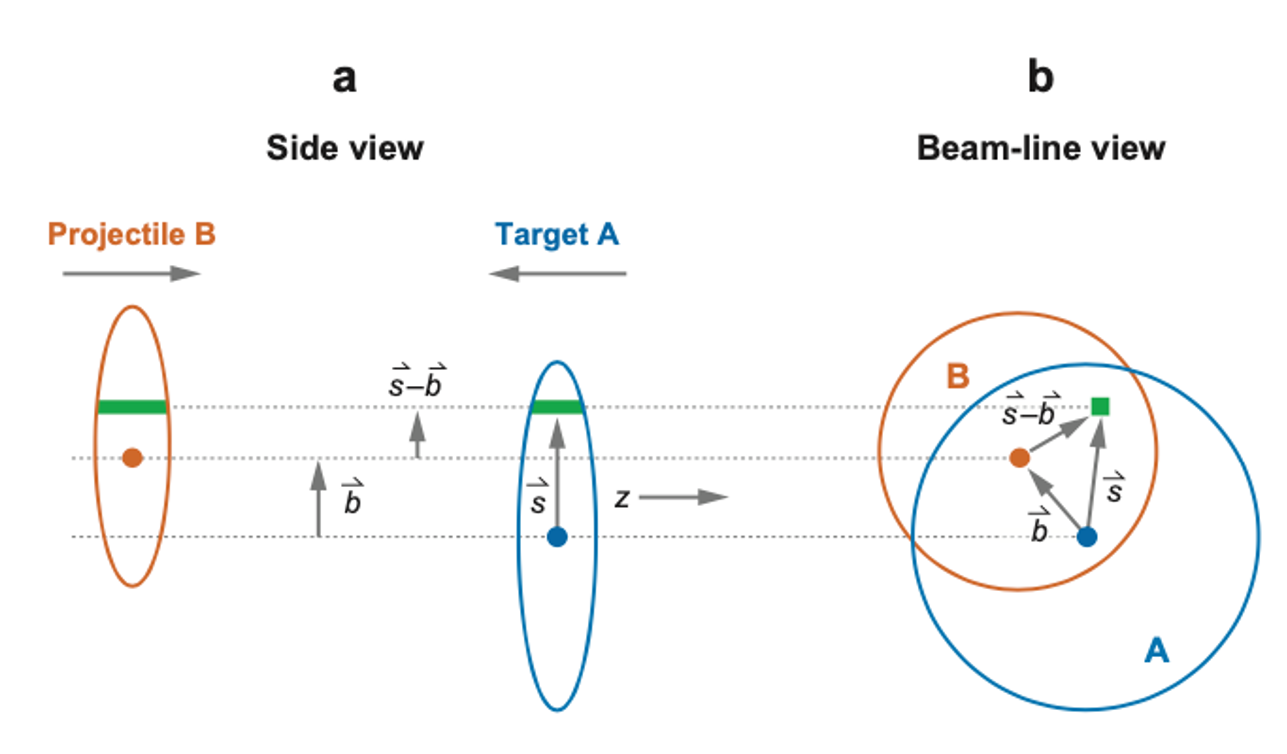
\includegraphics[width=0.7\textwidth,clip]{figures/Chapter1/ImpactParameter.png}
    \end{center}
    \caption[重离子对撞中的碰撞参数示意图]{重离子对撞中的碰撞参数示意图,其中图(a)为侧视图,图(b)为沿着束流方向视图。$\overrightarrow{b}$为碰撞参数,$\overrightarrow{s}$为Glauber模型中表示到核子中心距离的向量}
    \label{fig:ImpactParameter}
\end{figure}

\begin{figure}[htb]
    \begin{center}
    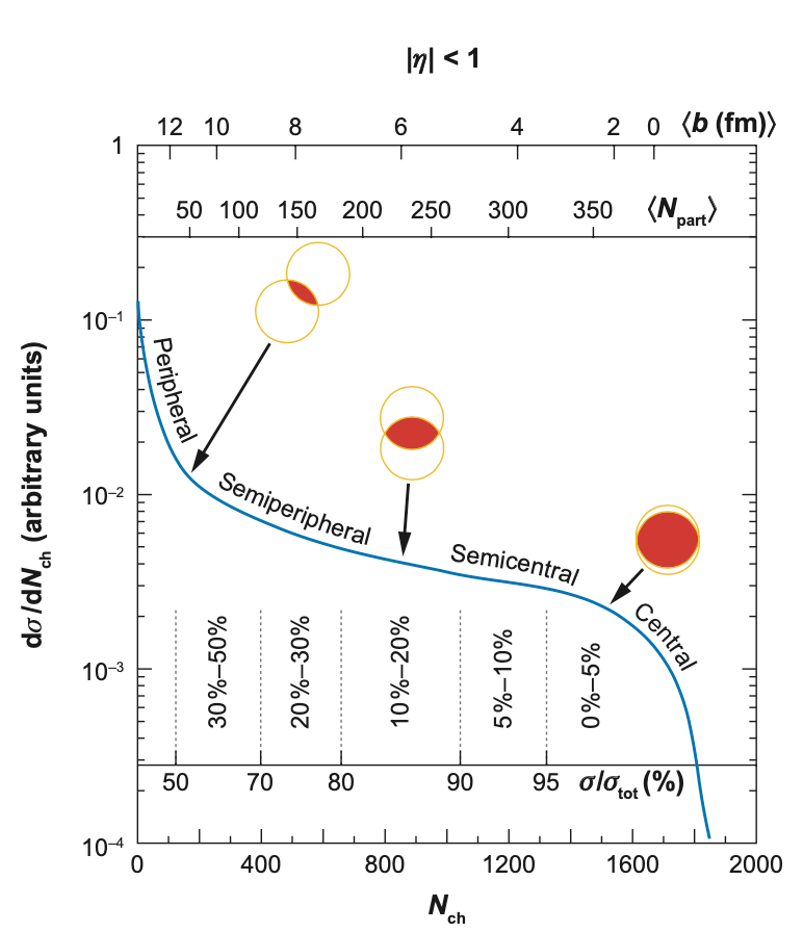
\includegraphics[width=0.6\textwidth,clip]{figures/Chapter1/Centrality.png}
    \end{center}
    \caption[中心度定义示意图]{Glauber模型中末态可观测的带电粒子径迹数和碰撞参数以及$N_{part}$的关系示意图,图中的值为定性的分布,并不是实际的测量值}
    \label{fig:Centrality}
\end{figure}

在一次重离子对撞发生以后所产生的QCD物质如何演化是重离子对撞物理中最为感兴趣的问题。对撞发生后的系统演化的示意图见图 \ref{fig:HIC}。在碰撞的早期发生的过程主要是核子和核子之间(或者说核子内的部分子)之间的散射过程,主要是有着小横动量转移的“软(soft)”过程。虽然数量较少但仍有一部分粒子发生了大横动量转移的过程(“硬(hard)”过程),产生了有着较高横动量($p_T$)的粒子,这些硬过程对我们的研究十分重要。碰撞发生的早期阶段被称作“预平衡”阶段,目前有多种理论模型来描述这个阶段,例如色玻璃凝聚模型(Color Glass Condensate, CGC),但我们对他们的动力学状态仍不是十分清楚。在碰撞发生后的大约 1 fm/c 之后,发生对撞的两个离子相互离开,但是在离子和离子重叠的区域沉积下了大量的能量,在这个时间段能量密度可以达到大约 $12 {\rm GeV/fm^{-3}}$,远大于强子内的能量密度,因此对撞中产生的夸克和胶子等难以保持束缚的强子态,从而组成一种新的物质的态,正是我们之前提到的夸克胶子等离子体。近些年来一些粘性流体力学的模型被用来描述QGP的性质并且取得了巨大的成功。

在之后,QGP向各个方向扩张同时冷却,当系统的温度接近$T_c \approx 150 {\rm MeV}$的时候系统开始冷却,首先夸克和胶子强子化生成各种强子,从夸克胶子等离子体相向强子气相转变,在这个过程中强子和强子之间仍可以发生非弹性散射,来改变粒子的种类。当强子的产额基本固定之后我们称这个状态为化学冻结(Chemical freeze-out)。 之后随着温度的进一步降低和系统的扩张,粒子之间的距离大于粒子散射的平均自由程时,粒子的动力学性质也几乎不再改变,这个状态被称为动力学冻结(Kinetic freeze-out)。动力学冻结发生后粒子的动量谱便不再改变并且自由地向各个方向飞出并被探测器探测到。

可以看到,整个QGP的演化时间极短,远小于现今的探测器可以做到的最小的时间分辨,这意味着我们需要从探测到的末态粒子来反推QGP的性质和初始状态,这就要求我们需要找到一些合适的物理探针来进行QGP的研究。从图 \ref{fig:HIC} 中可以看到,光子和电子可以在QGP演化的整个过程中产生,同时其又几乎不与强子物质发生反应,可以在末态被探测到并且受到较小的介质影响。是一个研究QGP的理想探针,将在下一节中进行详细的介绍。

% \begin{figure}[htb]
%     \begin{center}
%     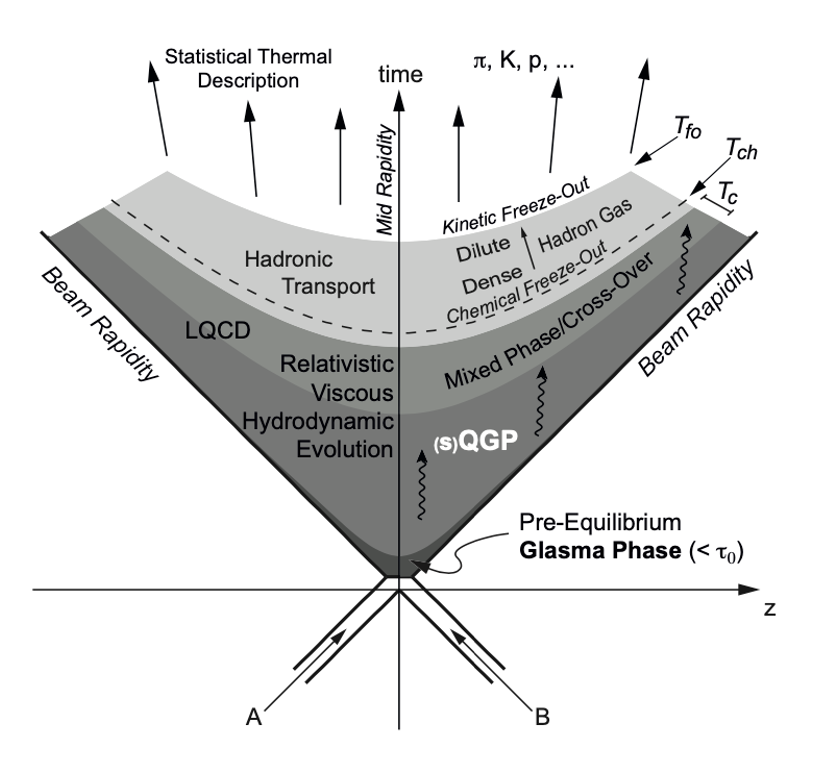
\includegraphics[width=0.8\textwidth,clip]{figures/Chapter1/HIC.png}
%     \end{center}
%     \caption[重离子对撞演化示意图]{一次重离子对撞发生后的系统演化的光锥示意图。主要的相和演化步骤以及对应的温度在图的右侧标出,成功的描述这种演化的模型在图的左侧被标出}
%     \label{fig:HIC}
% \end{figure}

\begin{figure}[htb]
    \begin{center}
    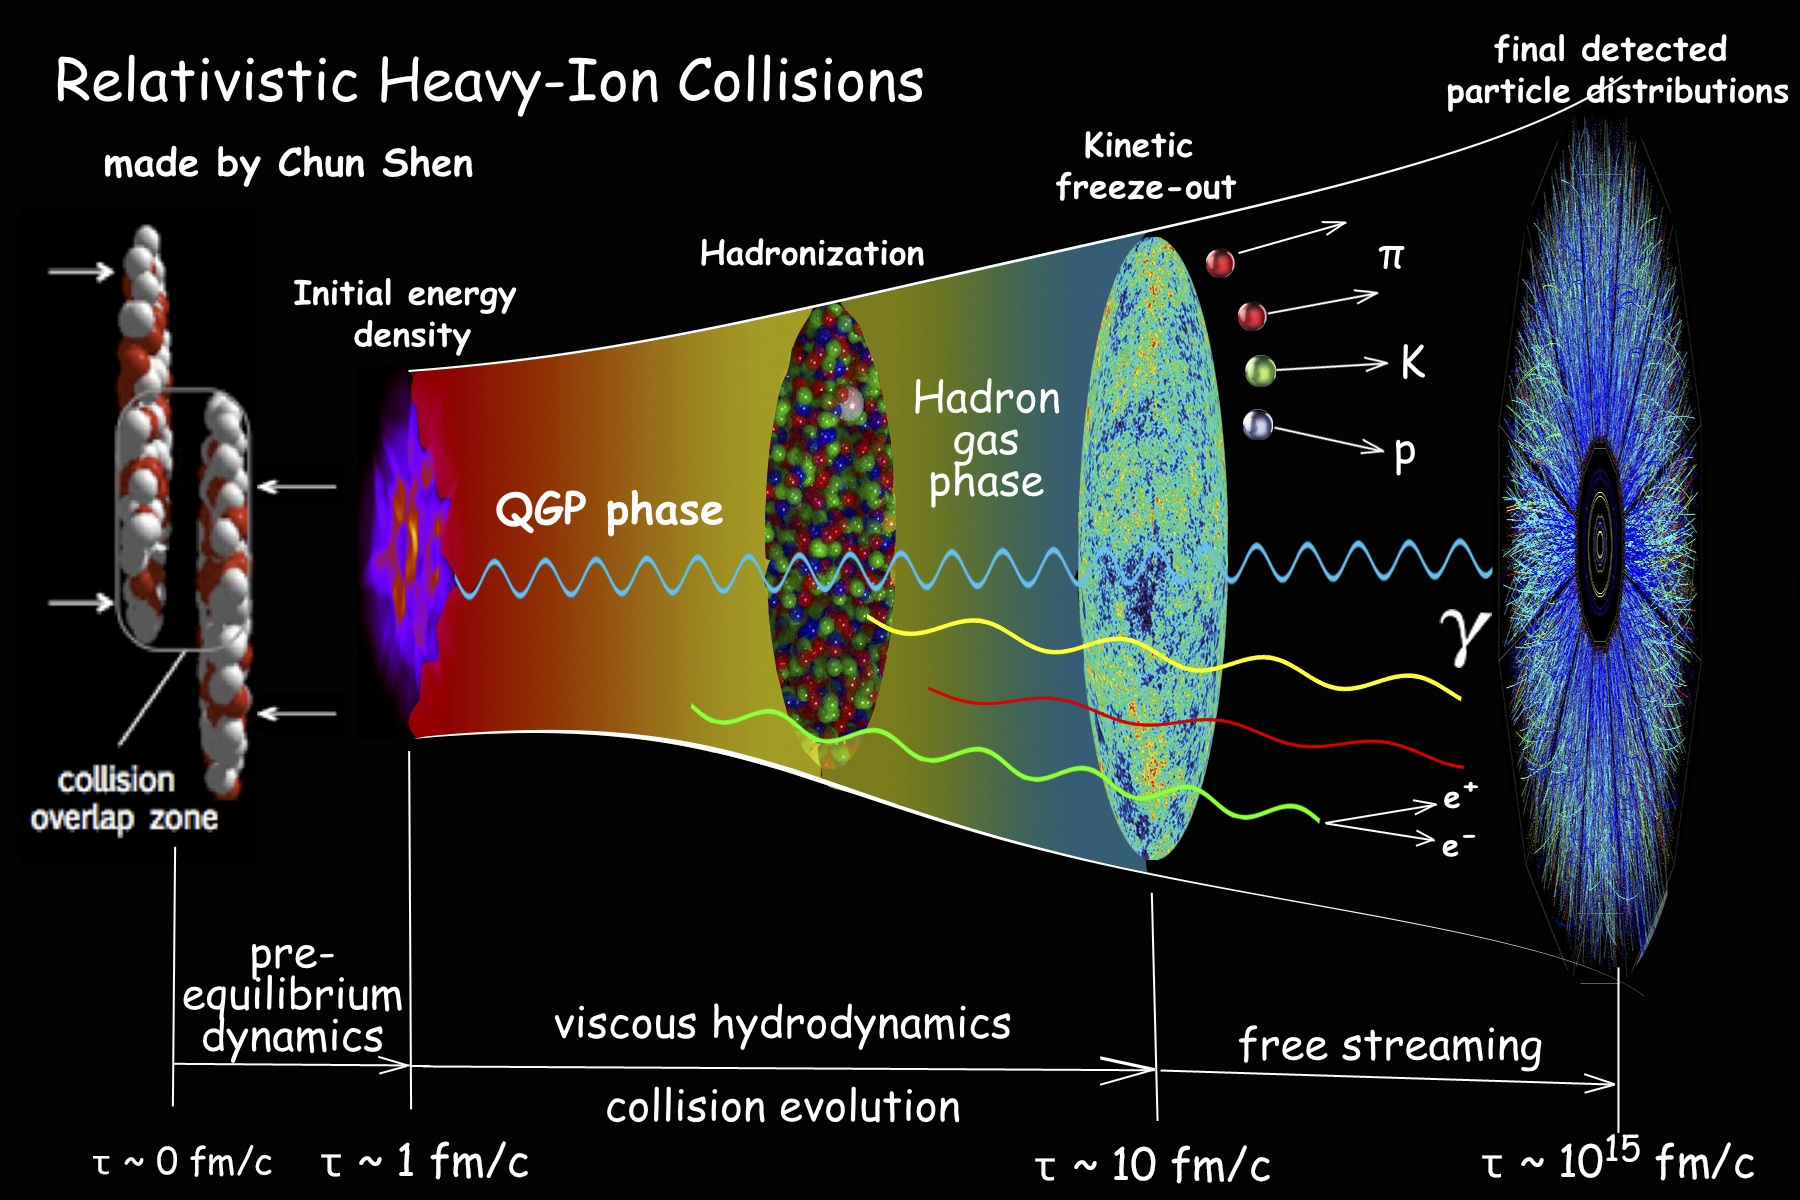
\includegraphics[width=0.8\textwidth,clip]{figures/Chapter1/little_bang-10wt2pd.jpeg}
    \end{center}
    \caption[相对论重离子演化示意图]{一次重离子对撞发生后的系统演化的示意图。图源https://u.osu.edu/vishnu/2014/08/06/sketch-of-relativistic-heavy-ion-collisions/}
    \label{fig:HIC}
\end{figure}
\section{相对论重离子对撞中的双轻子}

\subsection{相对论重离子对撞中的双轻子产生}

如上节中提到的那样,双轻子是如今相对论重离子对撞物理中一个很重要的电磁探针。通过双轻子我们可以有手段对介质初期的演化进行研究。对于双轻子来说,其不变质量谱是一个重要的物理观测量,在 不同的质量区间有着不同的产生机制。同时也是唯一一种可以直接观测QCD介质中介质修正谱方程(In-medium spectral function of QCD medium)的手段。接下来会对不同质量区间的的双轻子产生机制进行简要的介绍。

对于整个的双轻子不变质量谱,根据其产生机制和物理目标不同我们主要将其分为三个不同的质量区间,分别是低质量区间(Low Mass Region, LMR, $M_{ee} < M_{\phi}$ ),中等质量区间(Intermediate Mass Region, IMR, $M_{\phi} < M_{ee} < M_{J/\psi}$)和高质量区间(High Mass Region, HMR, $M_{J/\psi} < M_{ee}$)。双轻子的不变质量越重,其产生于系统演化的越早期。

\begin{figure}[htb]
    \begin{center}
    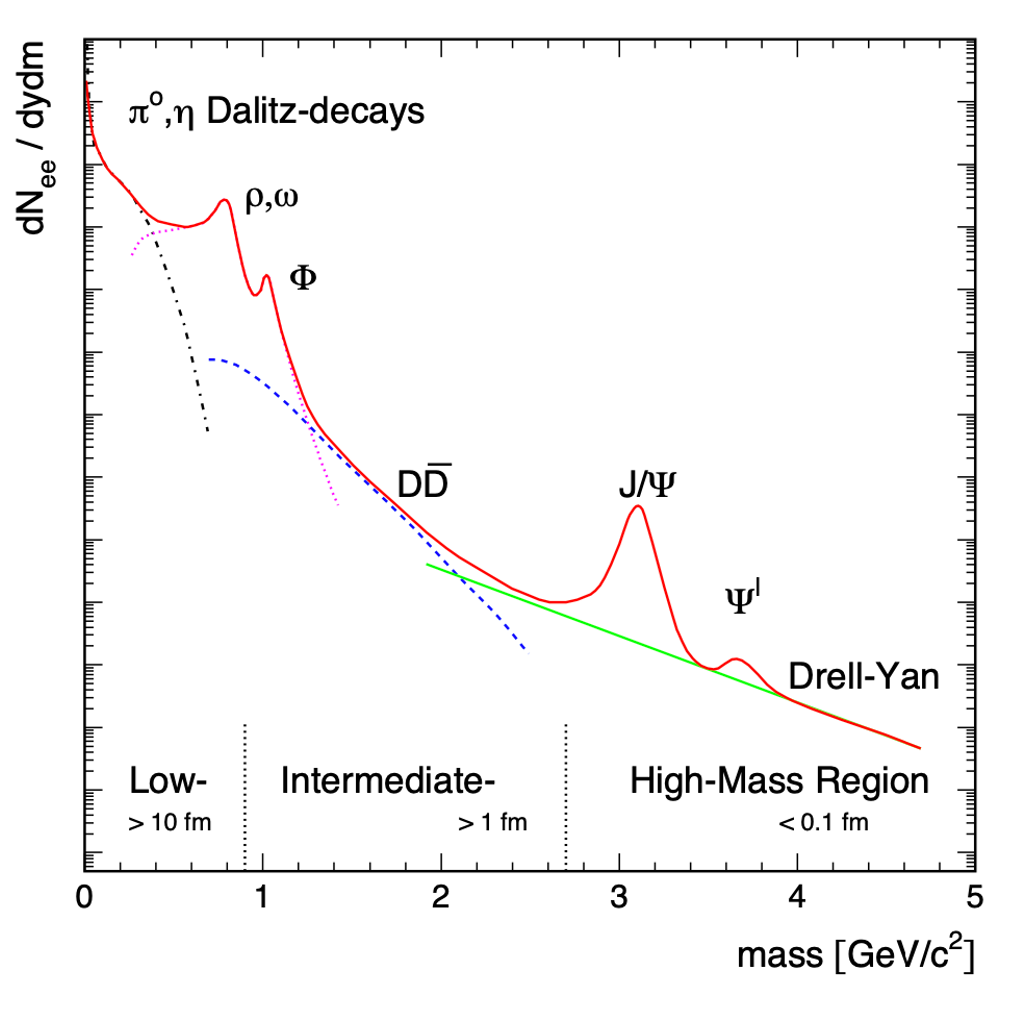
\includegraphics[width=0.8\textwidth,clip]{figures/Chapter1/DileptonSpectra.png}
    \end{center}
    \caption[双轻子不变质量谱示意图]{双轻子不变质量谱的质量区间划分和主要双轻子来源}
    \label{fig:DileptonSpectra}
\end{figure}

在高质量区间,双轻子主要来自于碰撞发生早期的部分子硬散射过程,例如Drell-Yan过程($q\bar{q} \rightarrow \gamma^*/Z \rightarrow l^{+}l^{-}$),重味夸克($b\bar{b}$)的半轻子衰变(semi-leptonic heavy flavor decays)以及重味夸克偶素的衰变($J/\psi, \psi(2S)$和$\Upsilon$)。

夸克偶素因为德拜屏蔽(Debye screening)在高温介质中解离成为夸克的过程被认为是夸克胶子等离子体存在的标志之一,因此夸克偶素在重离子对撞中的产额压低(suppression)是近些年来重离子对撞物理中一个十分令人感兴趣的课题。在离子-离子对撞中夸克偶素截面的核修正因子(Nuclear modification factor, $R_{AA}$)的测量中观测到了这种产额压低的存在。同时在RHIC上也观测到到了在前向快度区间($1.2 < |y| < 2.2$)相比于中间快度区间($|\eta <0.35|$)有着更强的产额压低,这意味着除了色屏蔽以外可能有着其他的机制对夸克偶素的产额有着影响。目前常见的理论有夸克偶素的重结合(recombination),冷核物质效应(Cold Nuclear Matter effect, (CNM))等。

在中等质量区间,双轻子的主要来源是c(charm)夸克的半轻子衰变以及夸克胶子等离子体的热辐射。在初始硬过程中产生的背对背的$c$和$\bar{c}$各自独立地强子化为$D$和$\bar{D}$介子,这些介子再进行半轻子衰变生成轻子。在强子化的过程中,这些强子继承了初始的$c\bar{c}$夸克对的关联性并将其带到了最后两个半轻子衰变的组成的轻子对当中。但因为介质对c夸克的影响,轻子和轻子之间的关联性将会发生一定的改变,对最后的不变质量谱产生影响。需要注意的是,在中等质量区间这部分来源于粲夸克半轻子衰变的双轻子产额远高于来源于夸克胶子等离子体热辐射的双轻子产额,这使得想要在此质量区间抽取来源于夸克胶子等离子体的热辐射的双轻子产额变得十分困难。给实验上测量带来了巨大的挑战。

对于小质量区间来说,双轻子对的主要来源是各种介子的衰变。在诸多介子的质量谱当中,$\rho^0$的质量谱在介质当中的演化是我们最感兴趣的部分。因为$\rho^0$的寿命为大约1.3 fm/c,远小于夸克胶子等离子体的寿命(在RHIC最高能量下的“中心”碰撞中大约为 10 fm/c),其不变质量谱明显地受到与介质相互作用的影响而发生了改变。这个相互作用主要来源于 $\pi^+ + \pi^- \leftrightarrow \rho$ 道的强耦合。这个不变质量谱的改变和手征对称性恢复相关。当手征对称性恢复发生的时候,两个不同的手征多重态的质量(如$\rho(770)$和$a_1(1260)$)发生简并。在实验上测量$a_1(1260)$的质量谱是很困难的,所以我们可以通过测量$\rho(770)$来对手征对称性的恢复进行测量。尽管相对于$a_1(1260)$的测量相对来说容易一些,在双轻子测量中测量$\rho(770)$质量谱依旧十分困难。这是因为在低质量区间除了由$\rho(770)$衰变产生的双轻子对,还有大量的来源于其他介子例如$\pi^0, \eta, \eta^\prime, \omega, \phi$等介子的衰变的双轻子对。为了抽取$\rho(770)$的不变质量谱,其他介子的不变质量谱需要通过某种手段从总的不变质量谱中扣除。对于所有已知产额的介子,我们可以通过模拟的方式来得到其在不同能量不同对撞系统下的不变质量谱,这样我们就可以从总的不变质量谱中扣除这些已知产额的介子的谱,剩下的便是我们想要测量的介子的质量谱。因为这种将多种介子的不变质量谱的模拟混合的方式就像调制鸡尾酒的时候将多种基酒混合在一起,这个模拟的方法被称作“强子衰变模拟(hadronic cocktail)”,将会在双轻子分析一章中进行详细的讨论。

综上所述,通过测量双轻子的不变质量谱可以达到丰富的物理目标,在过去的几十年中各个合作组在不同能量下对多种对撞系统进行了双轻子谱的测量,在接下来的一个小节中将对近些年来双轻子测量进行一个简单的回顾。
\subsection{双轻子测量历史}

在历史上,许多实验都进行过双轻子的测量,并且得到了十分显著的成果,在这一小节中将会对历史上的双轻子测量进行一个简要的回顾。

\subsubsection{NA45实验}
环形切伦科夫电子能谱仪(Cherenkov Ring Electron Spectrometer, CERES, aka NA45),即NA45实验是位于欧洲核子中心(Conseil Européenn pour la Recherche Nucléaire, CERN)的超级质子同步加速器(Super Proton Synchrotron, SPS)上的能谱仪。其可以用两个对称的环状切伦科夫探测器来对电子进行鉴别从而测量双电子谱。NA45首先对p+Be和p+Au系统低质量区间的双电子谱进行了测量,结果如图 \ref{fig:NA45pA} 所示。可以看到进行了背景扣除的双电子谱可以被强子衰变模拟很好地描述。同时这两个测量表明强子衰变模拟可以很好的描述初始的冷核物质效应。

\begin{figure}[htb]
    \centering
    \begin{subfigure}[b]{0.47\textwidth}
        \centering
        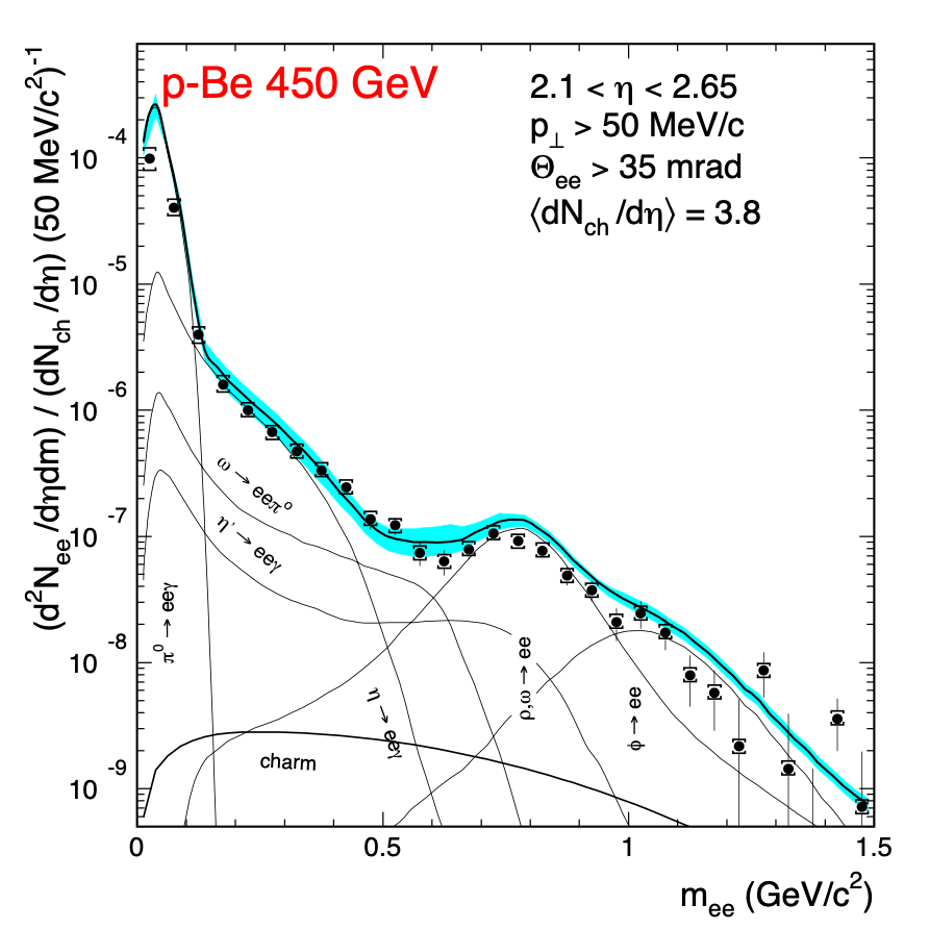
\includegraphics[width=\textwidth,clip]{figures/Chapter1/NA45pBe.png}
        \caption{}
        \label{fig:NA45pBe}
    \end{subfigure}
    \hfill
    \begin{subfigure}[b]{0.47\textwidth}
        \centering
        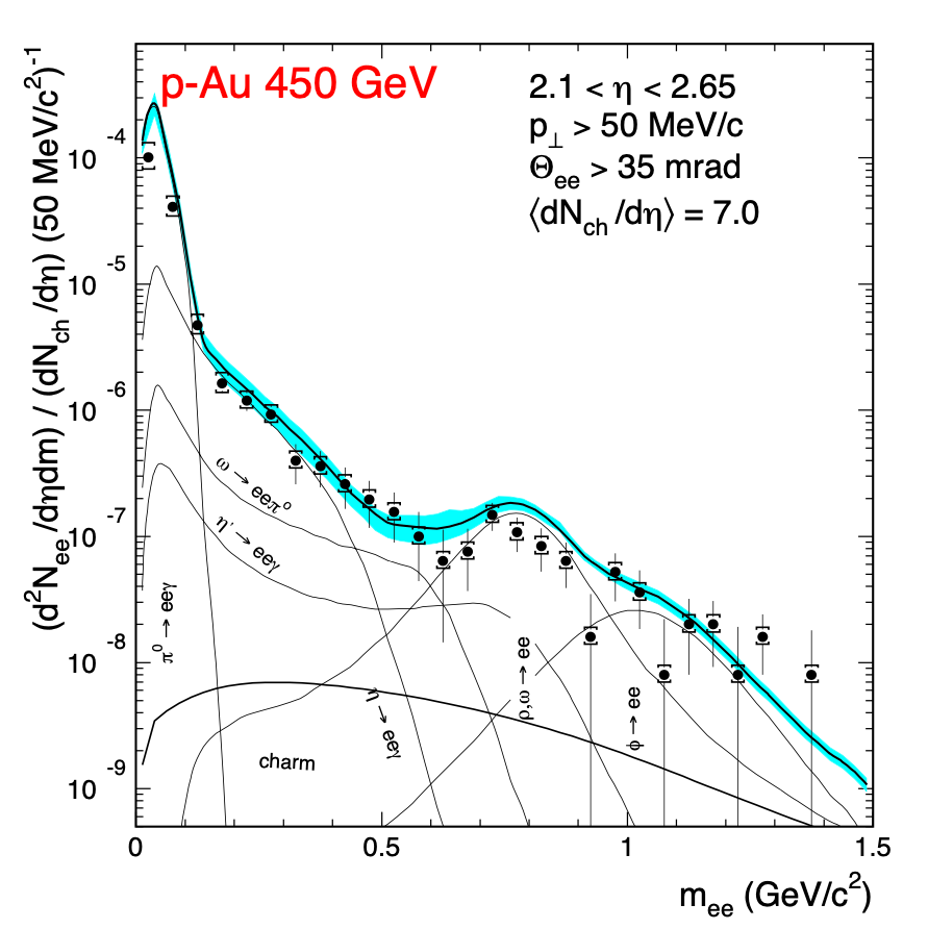
\includegraphics[width=\textwidth,clip]{figures/Chapter1/NA45pAu.png}
        \caption{}
        \label{fig:NA45pAu}
    \end{subfigure}
    \caption[NA45实验p+Be及p+Au对撞中低质量区间双电子谱]{NA45实验450 GeV p+Be \ref{fig:NA45pBe} 以及p+Au \ref{fig:NA45pAu} 对撞中的双电子谱。图中黑色实心圆点为数据点,黑线为强子衰变模拟结果。青色的error band代表了强子衰变模拟的系统误差。}
       \label{fig:NA45pA}
\end{figure}

之后NA45实验也对重离子对撞中的双电子谱进行了测量,图 \ref{fig:NA45SAu} 和图 \ref{fig:NA45PbAu} 分别展示了在200 AGeV 的硫-金对撞和 158 AGeV 铅-金对撞中的双电子谱。在这两个测量中可以看到数据点喝强子衰变模拟相比都有明显的额外产额增强。理论家们提出了一些模型来试图通过热辐射来解释这些额外产额,例如$\pi^+ + \pi^- \leftrightarrow \rho \rightarrow e^+ + e^-$过程。但当这些模型使用真空中的$\rho$质量谱的时候人们发现并不能很好的描述数据。这使得两种关于介质中的$\rho$不变质量谱的模型被提出来用以描述数据,分别是dorpping $\rho$ mass model 和 broadened $\rho$ model。这两种模型和数据的比较见图 \ref{fig:NA45PbAu}。但受限于统计,NA45的结果无法对这两种模型是否能很好的描述数据进行有效的分辨。这两种模型的比较直到后来NA60的更高精度双 \muon 谱测量结果出炉后才有了一个相对明确的结论。

\begin{figure}[htb]
    \centering
    \begin{subfigure}[b]{0.47\textwidth}
        \centering
        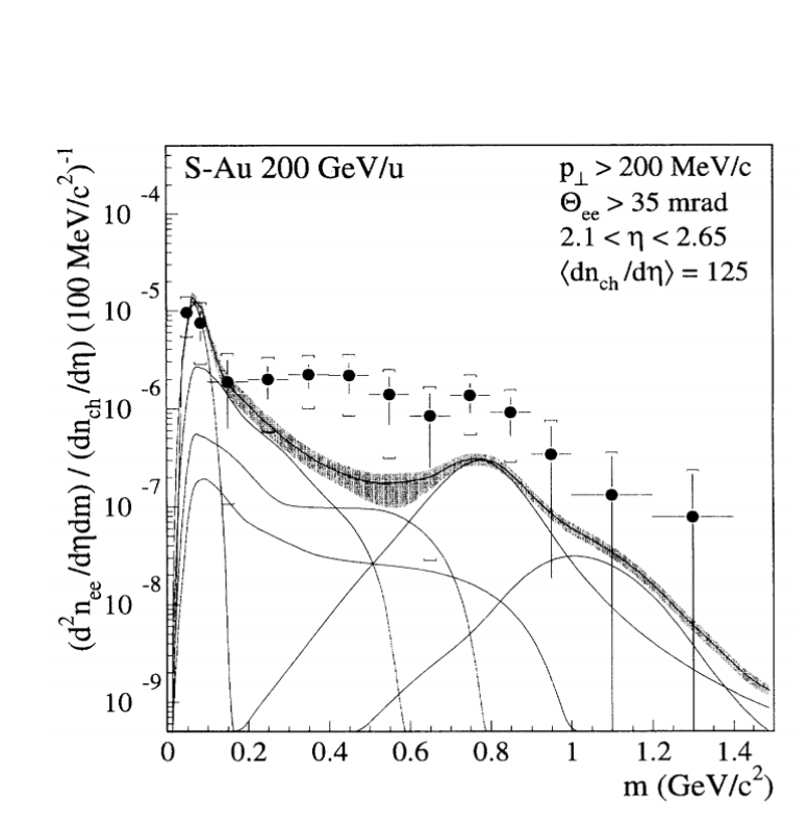
\includegraphics[width=\textwidth,clip]{figures/Chapter1/NA45SAu.png}
        \caption{}
        \label{fig:NA45SAu}
    \end{subfigure}
    \hfill
    \begin{subfigure}[b]{0.47\textwidth}
        \centering
        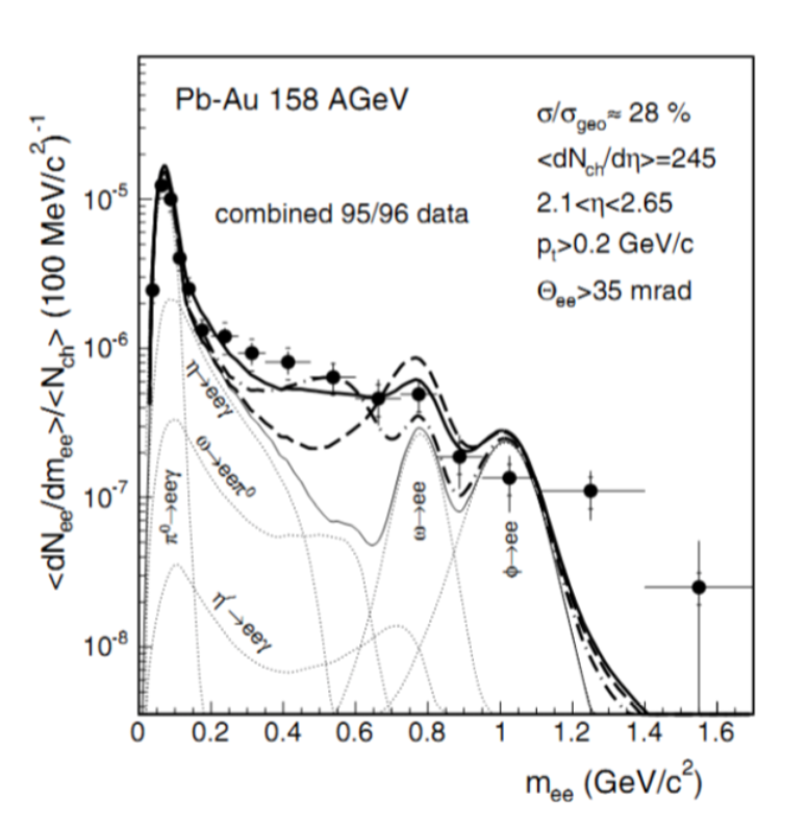
\includegraphics[width=\textwidth,clip]{figures/Chapter1/NA45PbAu.png}
        \caption{}
        \label{fig:NA45PbAu}
    \end{subfigure}
    \caption[NA45实验200 AGeV 硫-金及 158 AGeV 铅-金对撞中的双电子谱]{NA45实验中测得的200 AGev 硫-金对撞中的双电子谱\ref{fig:NA45SAu}和158 AGeV 铅-金对撞中的双电子谱\ref{fig:NA45PbAu}。右图中虚线为强子衰变模拟+真空中$\rho$双电子谱的模拟结果。两种不同的描述$\rho$的不变质量谱变化的模型一并被放入了图中,分别为在图中以点划线表示的dorpping $\rho$ mass model和以粗实线表示的broadened $\rho$ model。}
       \label{fig:NA45AA}
\end{figure}

\subsubsection{NA60实验}

NA60实验为超级质子同步加速器上的固定靶实验。因为NA60实验所拥有的高精度的 \muon 谱仪和顶点探测器,使得其有能力进行高质量分辨(~20 $\rm{MeV/c^20}$)和高位置分辨($ \sigma_x < 10 \mu m$,$\sigma_x < 15 \mu m$)的测量。基于高精度的实验设置,NA60可以有效的去除来自于弱衰变(例如 $\pi^{\pm} \rightarrow \mu^{\pm} + \nu_{\mu}(\bar{\nu}_{\mu})$和$K^{\pm} \rightarrow \mu^{\pm} + \nu_{\mu}(\bar{\nu}_{\mu})$)的背景和来源于重味半轻子衰变的 \muon 。NA60对 \sNN = 17.3 GeV 铟-铟对撞中的双 \muon 谱进行了测量,在全部中心度区间和“半中心”(semicentral)中心度区间的测量结果分别如图 \ref{fig:NA60NoCen} 和 \ref{fig:NA60SemiCentral}所示。
在“半中心”对撞的测量结果在扣除强子衰变模拟(不含 $\rho$)后和不同理论模型预测的$\rho$的不变质量谱进行了比较,因为该测量有着很高的精度,结果可以对理论模型的结果进行很好的约束。可以看到dropping $\rho$ 模型并不能描述数据而 broaden $\rho$ 模型可以在 $0.2 <  M_{\mu\mu} < 0.8~{\rm GeV/c^2} $的质量区间里很好的描述数据。
\begin{figure}[htb]
    \centering
    \begin{subfigure}[b]{0.47\textwidth}
        \centering
        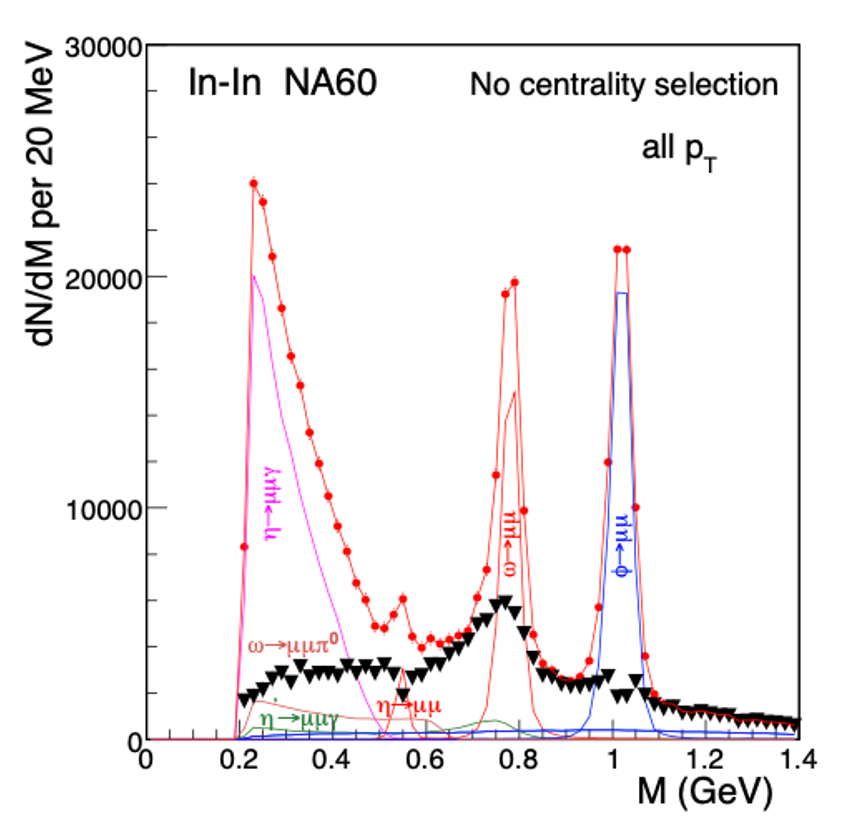
\includegraphics[width=\textwidth,clip]{figures/Chapter1/NA60NoCen.png}
        \caption{}
        \label{fig:NA60NoCen}
    \end{subfigure}
    \hfill
    \begin{subfigure}[b]{0.47\textwidth}
        \centering
        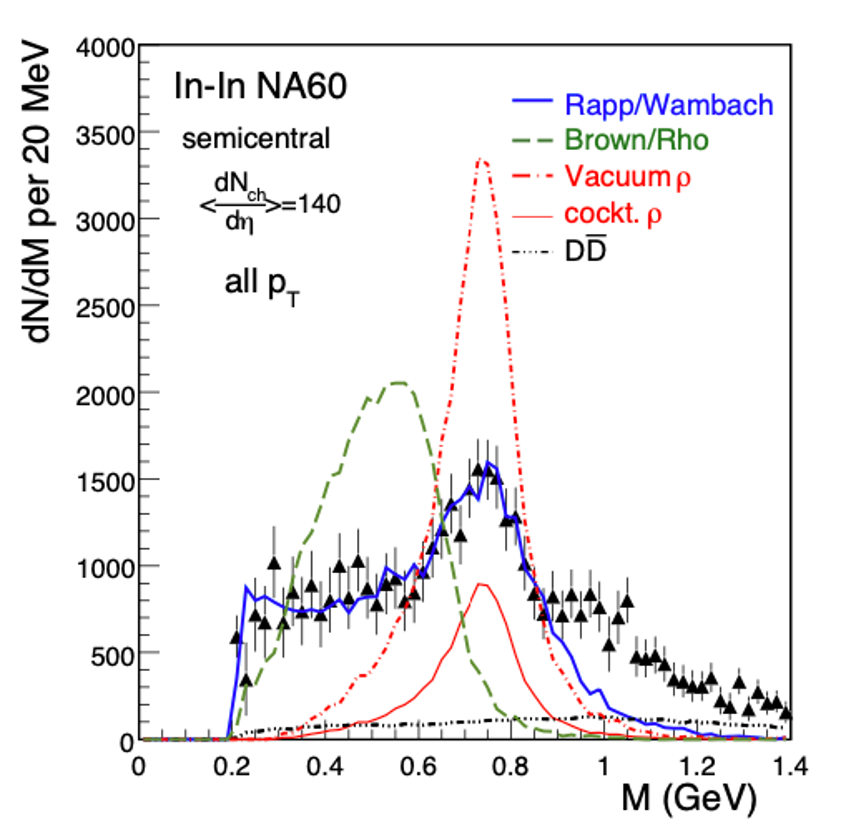
\includegraphics[width=\textwidth,clip]{figures/Chapter1/NA60SemiCentral.png}
        \caption{}
        \label{fig:NA60SemiCentral}
    \end{subfigure}
    \caption[NA60实验\sNN = 17.3 GeV 铟-铟对撞中的双 \muon 谱]{NA60实验\sNN = 17.3 GeV 铟-铟对撞中的双 \muon 谱。左图中未进行中心度筛选的双 \muon 谱,其中红色圆点为未扣除强子衰变模拟的双 \muon 谱,黑色三角为扣除强子衰变模拟后的双 \muon 谱。右图为扣除强子衰变模拟后在“半中心”中心度下的双 \muon 谱。来自不同模型预测的 $\rho$ 的产额在途中以不同形式的线标出。}
       \label{fig:NA60DiMuon}
\end{figure}

在更高的质量区间($M_{\mu\mu} > 0.8~{\rm GeV/c^2}$),双 \muon 的额外产额并不能被任何一种有关 $\rho$ 不变质量谱在介质中的修正模型来描述。在高精度的顶点测量探测器的帮助下NA60实验可以对双轻子的额外产额来源进行分析。经过分析,重味夸克的半轻子衰变和Drell-Yan过程被认为不是额外产额的主要来源。因为统计量足够,NA60进一步对不同的质量区间进行了$m_{T}~(m_{T} = \sqrt{p_T^2 + m^2})$谱的研究。在不同的质量区间用一个指数分布来拟合$m_T$谱,拟合方程为:$1/m_{T}*dN/dm_{T} \propto exp(-m_{T}/T_{eff})$。其中的反斜率参数$T_{eff}$可以被解释为介质的有效温度。在不同质量区间中的有效温度的拟合如图 \ref{fig:NA60T}所示。$T_{eff}$在大约1 GeV处的突然降低表明用强子产生并不能很好的解释在中等质量区间的双轻子额外产额,更自然的解释是这部分额外产额来源于介质的热辐射。

\begin{figure}[htb]
    \begin{center}
    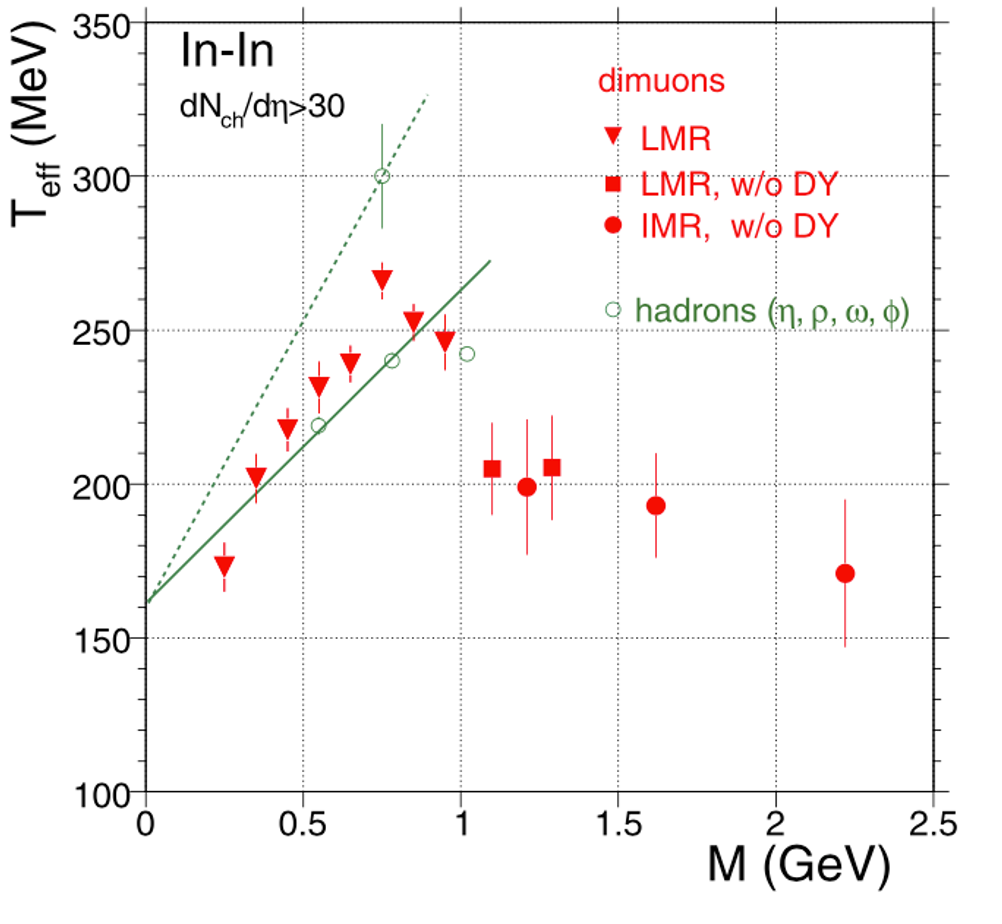
\includegraphics[width=0.75\textwidth,clip]{figures/Chapter1/NA60T.png}
    \end{center}
    \caption[NA60不同质量区间的有效温度测量结果]{NA60实验在不同质量区间下用$exp(-m_{T}/T_{eff})$拟合$m_T$谱得到的有效温度参数结果,并且与从强子谱得到的结果(绿色空心点)进行比较}
    \label{fig:NA60T}
\end{figure}

\subsubsection{PHENIX实验}

在RHIC上的双轻子测量主要由PHENIX(The Pioneering High Energy Nuclear Interaction eXperiment, PHENIX)实验和STAR(Solenoidal Tracker at RHIC)实验完成。

首先我们对PHENIX实验的双轻子测量结果进行一个简要的回顾。PHENIX实验是RHIC的两个大型粒子物理实验之一,其可以对中等快度区间内一定方位角的粒子进行测量,其探测器设计参数见参考文献[]。PHENIX首先对\sNN = 200 GeV质子-质子对撞中的双电子谱进行了测量,结果如图 \ref{fig:PHENIXpp} 所示。数据和强子衰变模拟的数据在误差范围内符合的很好,证明质子-质子对撞可以作为我们研究金-金对撞中的双电子谱时的基线。随后PHENIX也对 \sNN = 200 GeV 金-金对撞中的双电子谱进行了测量。在不同中心度下的结果如图 \ref{fig:PHENIXAuAu} 所示。在相对中心的对撞中心度下均观察到了在低质量区间($ 0.15 < M_{ee} < 0.75~{\rm GeV/c^2}$)相比于强子衰变模拟的产额增强。从图中也可以看到随着对撞接近中心对撞,这种产额增强的程度越来越高。这种增强和之前的预期相符。同时在低质量区间($M_{ee} < 0.3~{\rm GeV/c^2}$)和相对较高的横动量区间($ 1 < p_T < 5 ~{\rm GeV/c^2}$)的区间在质子-质子和金-金对撞中都观测到了产额的增强,在这个区间内的额外产额和质量的依赖关系和直生虚光子的产生的预测相符合。PHENIX也对直生虚光子进行了测量,但在本文中不进行详细的讨论,可参见参考文献[]。

\begin{figure}[htb]
    \centering
    \begin{subfigure}[b]{0.45\textwidth}
        \centering
        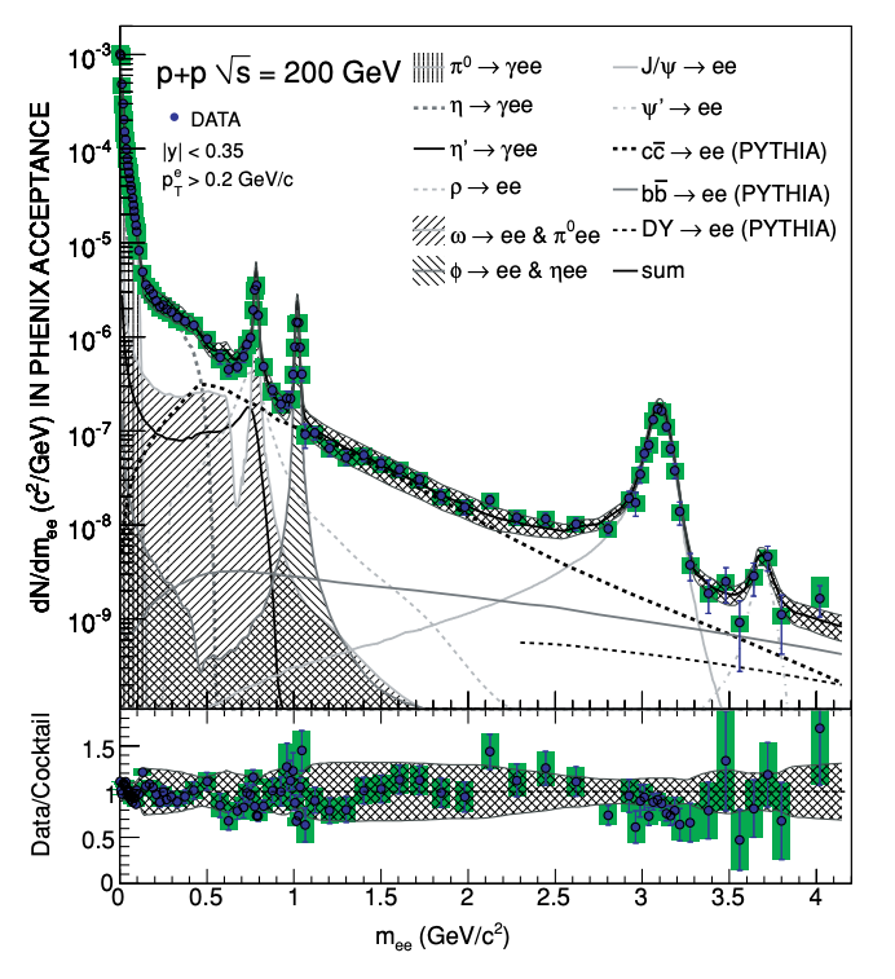
\includegraphics[width=\textwidth,clip]{figures/Chapter1/PHENIXpp.png}
        \caption{}
        \label{fig:PHENIXpp}
    \end{subfigure}
    \hfill
    \begin{subfigure}[b]{0.45\textwidth}
        \centering
        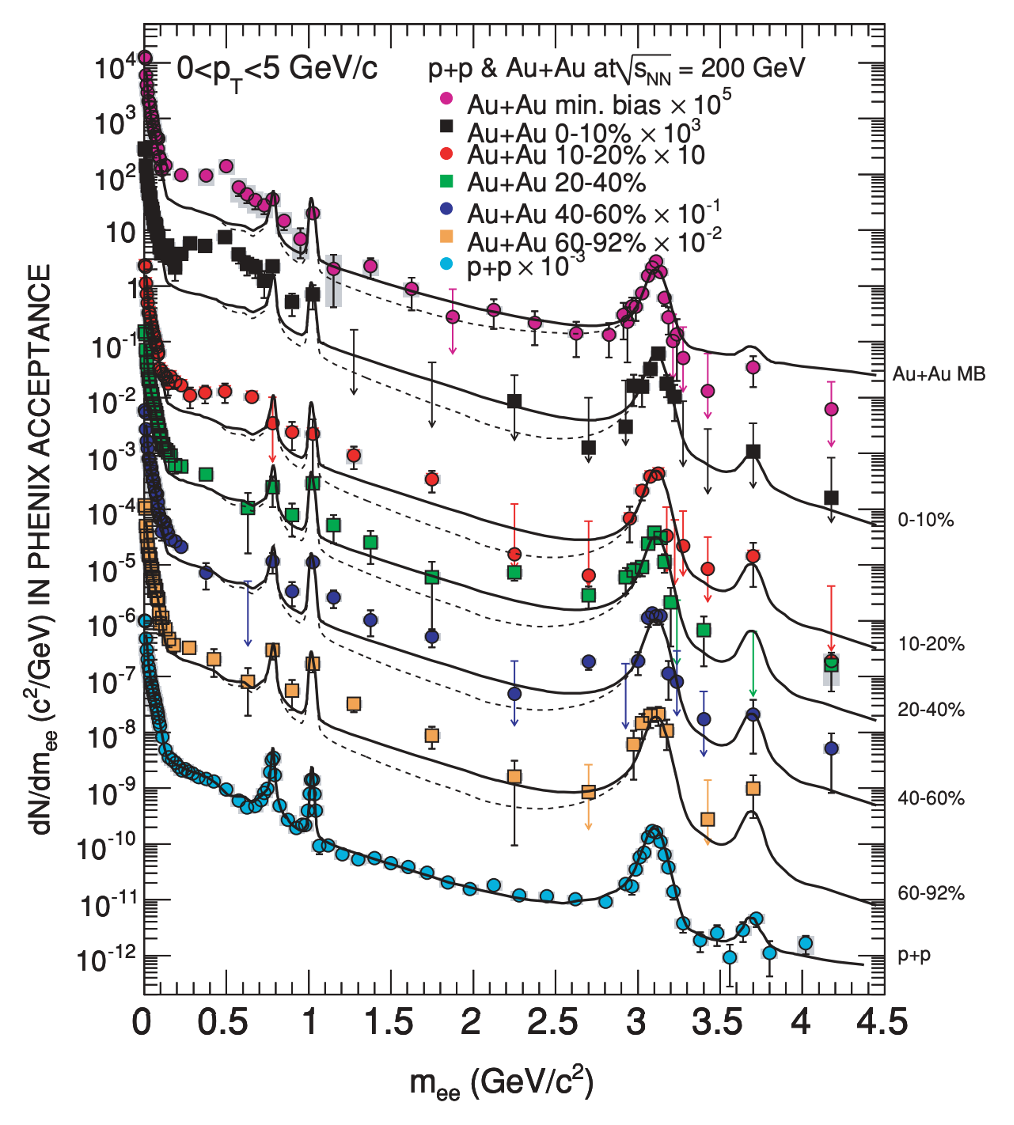
\includegraphics[width=\textwidth,clip]{figures/Chapter1/PHENIXAuAu.png}
        \caption{}
        \label{fig:PHENIXAuAu}
    \end{subfigure}
    \caption[PHENIX实验 \sNN = 200 GeV 质子-质子和金-金对撞中的双电子谱测量结果]{PHENIX实验在其接收度下的 \sNN = 200 GeV 质子-质子和金-金对撞中的双电子谱测量结果。左图为质子-质子对撞中的双电子谱测量结果。测量结果与强子衰变模拟的结果进行比较,强子衰变模拟的不同双电子源在图中已经标出。右图为\sNN = 200 GeV质子-质子和金-金对撞中不同中心度下的双电子谱。}
       \label{fig:PHENIXDiElectron}
\end{figure}

\subsubsection{STAR实验}

作为RHIC上的另一个大型粒子物理实验,STAR实验也对不同对撞系统和不同对撞能量中的双轻子谱进行了测量。在STAR的主径迹探测器时间投影室(Time Projection Chamber, TPC)和飞行时间探测系统(Time of Flight, TOF)的帮助下,STAR有能力获得高电子纯度的数据样本。以金-金 \sNN = 200 GeV 对撞的数据为例,其可获得电子纯度最高为94.6 ± 2 \%的数据样本。

和PHEINX实验类似,为了给离子-离子对撞中的测量定下一条好的基线,STAR的双轻子测量也是从质子-质子对撞开始的。STAR的首个双轻子测量结果基于2009年采集的质子-质子对撞数据,结果如图 \ref{fig:STARpp}所示。和PHENIX饰演的结果类似,强子衰变模拟也可以很好的描述测量到的双轻子谱。其中源自c夸克双电子模拟结果由PYTHIA6模拟得到。之后STAR合并2010和2011年两年的金-金 \sNN = 200 GeV下的数据进行了双电子谱的测量,如图 \ref{fig:STARAuAu}所示。在 $\rho$ 的质量区间($0.3 < M_{ee} < 0.76 ~{\rm GeV/c^2}$)STAR观测到了相比于强子衰变模拟1.76 ± 0.06 (stat) ± 0.26 (systematic) ± 0.29 (cocktail)倍的产额增强。STAR在 \sNNerbai 金金对撞中的测量结果在统计误差范围内和PHENIX合作组的测量结果可以符合,并且对于额外产额也和几种不同的理论模型进行了比较。

\begin{figure}[htb]
    \centering
    \begin{subfigure}[b]{0.43\textwidth}
        \centering
        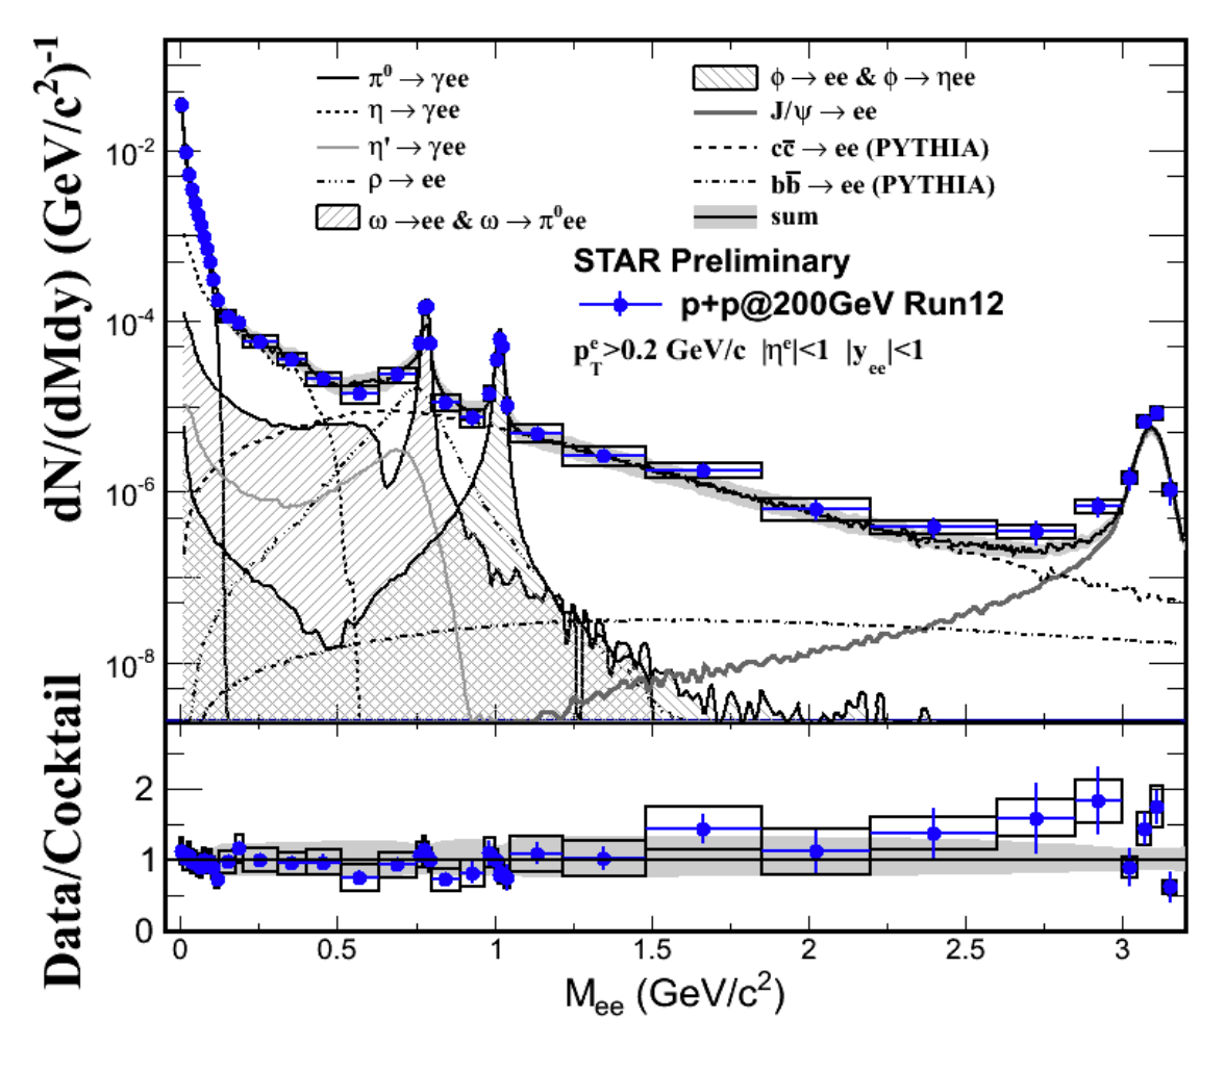
\includegraphics[width=\textwidth,clip]{figures/Chapter1/STARpp.png}
        \caption{}
        \label{fig:STARpp}
    \end{subfigure}
    \hfill
    \begin{subfigure}[b]{0.43\textwidth}
        \centering
        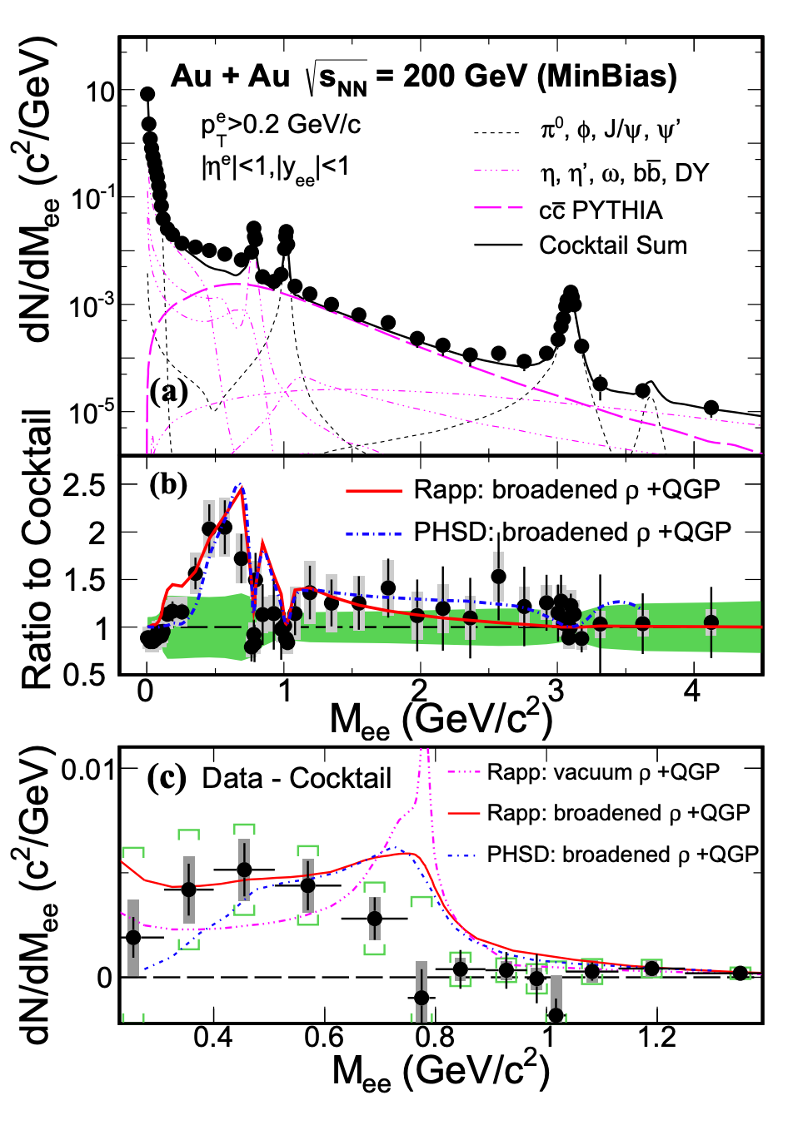
\includegraphics[width=\textwidth,clip]{figures/Chapter1/STARAuAu200.png}
        \caption{}
        \label{fig:STARAuAu}
    \end{subfigure}
    \caption[STAR实验 \sNN = 200 GeV 质子-质子和金-金对撞中的双电子谱测量结果]{STAR实验在其接收度下的 \sNN = 200 GeV 质子-质子和金-金对撞中的双电子谱测量结果。左图为质子-质子对撞中的双电子谱测量结果。测量结果与强子衰变模拟的结果进行比较,强子衰变模拟的不同双电子源在图中已经标出。右图的(a)部分为\sNN = 200 金-金对撞中0-80\%中心度下的双电子谱和强子衰变模拟的结果。(b)部分为数据和强子衰变模拟的比值,(c)部分为额外产额(data-cocktail),并且和几种不同的理论模型相比较}
       \label{fig:STARDiElectron}
\end{figure}

随着能量扫描(Beam Energy Scan)的进行,STAR在多个能量下对金-金对撞中的双电子谱进行了系统的测量。图展示了STAR在 \egyfive 金-金对撞中 0-80\%中心度下的双电子谱。在多个能量下STAR都观测到了在 $\rho$ 质量区间的产额增强。同时STAR在 \sNN = 19.6 GeV的金-金对撞中经过$dN_{ch}/d\eta$归一化和STAR接收度修正后额外产额和 NA60 \sNN = 17.3 GeV 铟-铟对撞下的额外产额可以很好的符合,结果见图 \ref{fig:STAR19p6}。理论模型也可以很好的描述\sNN = 19.6 GeV下双轻子额外产额。

\begin{figure}[htb]
    \begin{center}
    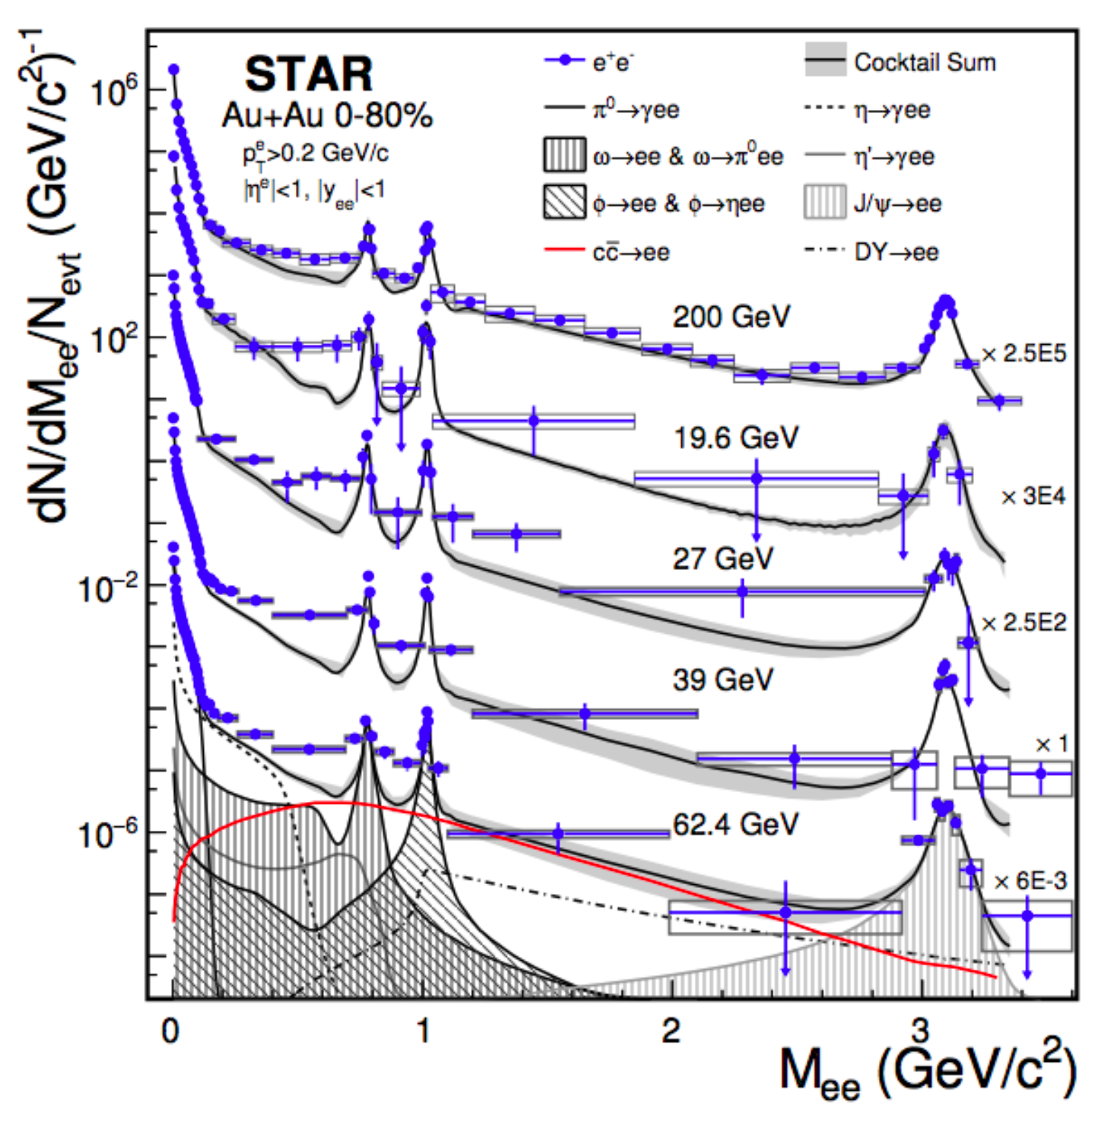
\includegraphics[width=0.6\textwidth,clip]{figures/Chapter1/STARBES.png}
    \end{center}
    \caption[STAR实验 \egyfive 下的双轻子谱]{STAR实验 \sNN = 19.6,27,39,62.4和200GeV下的双轻子谱。系统误差和统计误差分别用方框和竖线列出。图中仅展示了 \sNN = 62.4 GeV的强子衰变模拟结果,其余结果均与各自能量下的强子衰变模拟结果进行比较。}
    \label{fig:STARBES}
\end{figure}

\begin{figure}[htb]
    \begin{center}
    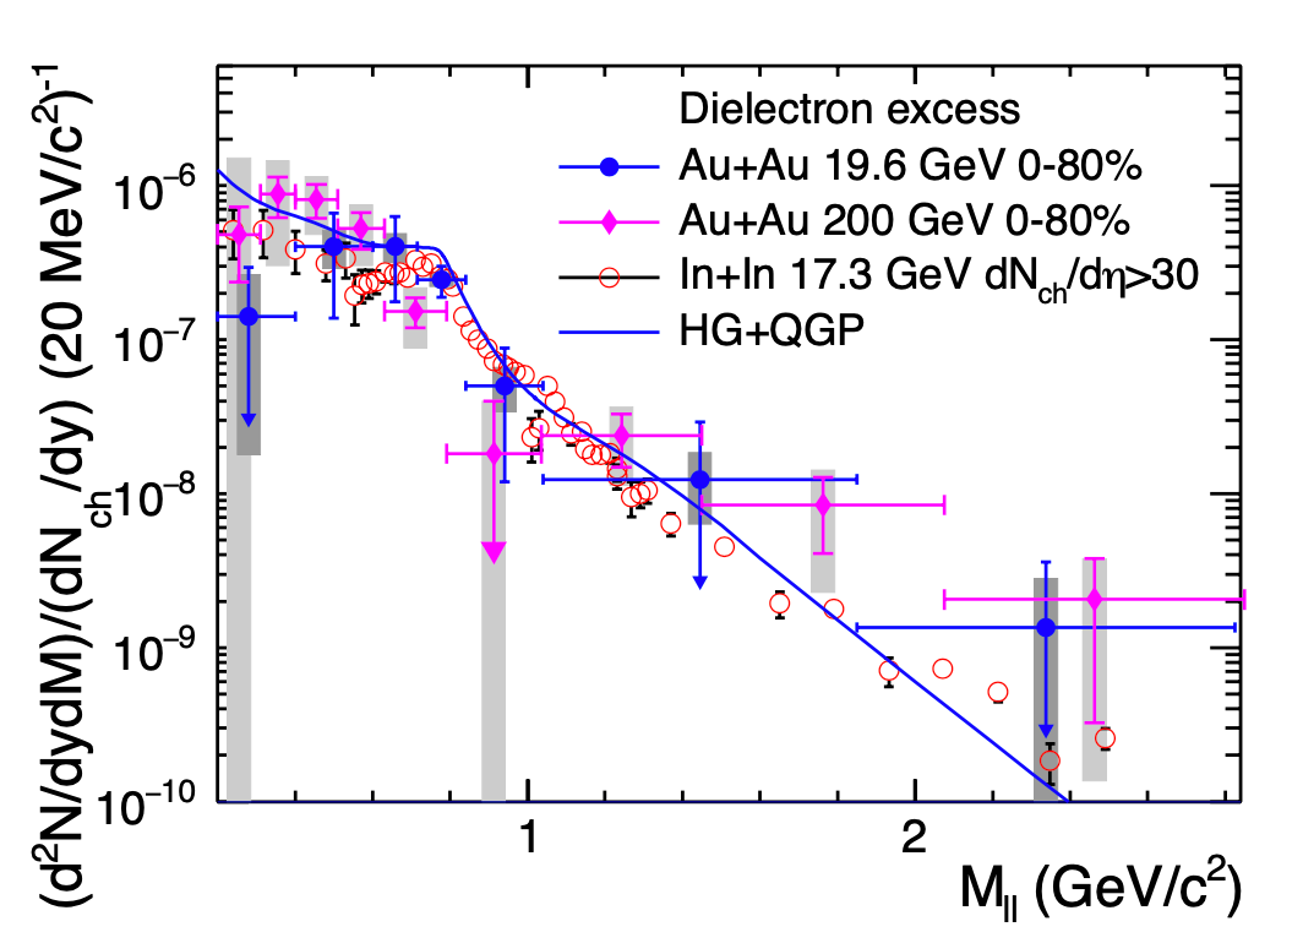
\includegraphics[width=0.6\textwidth,clip]{figures/Chapter1/STAR19p6.png}
    \end{center}
    \caption[STAR实验 \sNN = 19.6和200 GeV 的双轻子谱额外产额和NA60的额外产额比较]{STAR实验 \sNN = 19.6和200 GeV 的双轻子谱额外产额在经过中间快度区间的带电粒子多重数归一化和STAR接收度修正后和NA60的额外产额比较。蓝色实线为包含强子气(Hadron Gas)中broaden $\rho$ 和 QGP热辐射贡献的模型计算结果。 }
    \label{fig:STAR19p6}
\end{figure}

在 \sNN = 200GeV 的情况下,虽然有很高的统计但是随着对撞能量的增加,来源于重味夸克的双轻子在中等质量区间所占的产额比例逐渐增加,导致STAR在\sNN = 200GeV 双轻子测量中难以去抽取来自夸克胶子等离子体的热辐射产额。而在 \sNN = 19.6, 27, 39, 62.4 GeV 几个对撞能量下,虽然重味夸克的截面相比于\sNN = 200GeV 有所降低,但受限于统计也无法在中等质量区间进行热辐射产额的抽取。2017年STAR采集了大约12亿个\sNN = 54.4 GeV的金-金对撞事例。使得STAR有足够的统计在较低的对撞能量下尝试抽取来自于热辐射的双轻子产额。






